%% LyX 2.2.2 created this file.  For more info, see http://www.lyx.org/.
%% Do not edit unless you really know what you are doing.
\documentclass[11pt,english]{beamer}
\usepackage{enumerate}

\usepackage{mathptmx}
\usepackage[T1]{fontenc}
\usepackage[utf8]{inputenc}
\setlength{\parskip}{\smallskipamount}
\setlength{\parindent}{0pt}
\usepackage{url}
\usepackage[authoryear]{natbib}
\usefonttheme[onlymath]{serif} % para las fuentes de las ecuaciones
\makeatletter
\usepackage{amsmath,amssymb,amsthm}
\usepackage{graphicx}
\usepackage{xcolor} % para colorear textos con \textcolor o \color
\usepackage{hyperref}
\usepackage{times}
\usepackage{array}
\usepackage{multicol}
\usepackage{longtable}
\usepackage{float} % para usar comando [H] en tablas y gr\'aficas
\usepackage{xcolor}% para modificar el color de la presentacion y del texto
\usepackage{colortbl} % para tablas de Kable
\usepackage{booktabs} % Para toprule: To thicken table lines 
\usepackage[nogin]{Sweave} % elimina el tamaño por default de las figuras de sweave
\usepackage{natbib}
\bibliographystyle{agsm}
% \usepackage[inline]{enumitem} % para enumerar dentro de un paragrafo
\usepackage{rotating} % para rotar nombres de columnas

\usepackage{graphicx}
\usepackage{subcaption}
\usepackage[strings]{underscore}
\usepackage{tabularx}



%%%%%%%%%%%%%%%%%%%%%%%%%%%%%% LyX specific LaTeX commands.
\providecommand{\LyX}{L\kern-.1667em\lower.25em\hbox{Y}\kern-.125emX\@}

%%%%%%%%%%%%%%%%%%%%%%%%%%%%%% Textclass specific LaTeX commands.
 % this default might be overridden by plain title style
 \newcommand\makebeamertitle{\frame{\maketitle}}%
 % (ERT) argument for the TOC
 \AtBeginDocument{%
   \let\origtableofcontents=\tableofcontents
   \def\tableofcontents{\@ifnextchar[{\origtableofcontents}{\gobbletableofcontents}}
   \def\gobbletableofcontents#1{\origtableofcontents}
 }
\newcommand{\code}[1]{\texttt{#1}}

%%%%%%%%%%%%%%%%%%%%%%%%%%%%%% User specified LaTeX commands.
\usetheme{Warsaw}
% or ...

\setbeamercovered{transparent}
% or whatever (possibly just delete it)

\usepackage[T1]{fontenc}

\makeatother

\usepackage{babel}
\usepackage{listings}
\renewcommand{\lstlistingname}{\inputencoding{latin9}Listing}
\newtheorem{ejem}{\textbf{Ejemplo}}[section]
\begin{document}
\Sconcordance{concordance:1_panorama_Diapositivas.tex:1_panorama_Diapositivas.rnw:1 %
50 1 1 4 77 1 1 17 1 2 16 1 1 20 1 2 17 1 1 8 1 2 22 1 1 18 1 2 21 1 1 %
15 1 2 25 1 1 25 1 2 12 1 1 52 1 2 298 1 1 38 1 2 82 1 1 17 11 0 1 2 20 %
1 1 5 33 0 1 2 14 1 1 7 1 2 5 1 1 5 1 2 84 1 1 9 33 0 1 2 12 1 1 88 1 2 %
16 1 1 39 1 2 146 1 1 19 18 0 1 3 5 1 1 10 17 0 1 2 9 1 1 74 1 2 9 1 1 %
8 18 0 1 2 7 1 1 62 1 3 6 1 1 5 5 1 2 2 115 1 1 5 1 6 5 1 1 39 1 2 9 1 %
1 3 1 2 103 1 1 4 1 6 3 1 1 9 48 0 1 2 4 1 1 48 7 1 2 2 7 1 2 2 4 1 2 2 %
4 1 2 2 4 1 2 2 4 1 2 2 4 1 2 2 1 1 1 4 5 1 1 6 1 2 10 1 1 21 1 2 5 1}



\title{Estadística Descriptiva Multivariada\\
\small Métodos multivariados aplicados (Aprendizaje no supervisado)
}

\subtitle{Contexto de la estadística descriptiva multivariada, contenido del curso y criterios de calificación}

\author{Jimmy A Corzo S\inst{1} \inst{2}}

\institute[Profesor Titular]{\inst{1}Profesor Titular\\
Departamento de Estadística\and \inst{2}Facultad de ciencias\\
Universidad Nacional de colombia}

% \date[2023]{Métodos multivariados aplicados \LyX{} Contenido y criterios de calificación}

\makebeamertitle

%\pgfdeclareimage[height=0.5cm]{institution-logo}{institution-logo-filename}

%\logo{\pgfuseimage{institution-logo}}

\AtBeginSubsection[]{

  \frame<beamer>{ 

    \frametitle{Outline}   

    \tableofcontents[currentsection,currentsubsection] 

  }

}

%------------------------------------------------------------
% (En el preámbulo de su Beamer .Rnw asegúrese de tener)
% \usepackage{graphicx}
% \usepackage{amsmath,amssymb}
%------------------------------------------------------------

%============================================================
\begin{frame}
\large{\textcolor{blue}{Panorama\\La Estadística Descriptiva Multivariada (EDM) en el contexto moderno del aprendizaje estadístico no supervisado}}
\end{frame}

\begin{frame}{Aprendizaje Estadístico Supervisado: el problema}
\setkeys{Gin}{height=0.5\textheight, keepaspectratio}
\small
\textbf{Objetivo.} Predecir una variable respuesta $Y$ a partir de predictores
$X_1,\ldots,X_p$ mediante un modelo
\[
Y = f(X_1,\ldots,X_p).
\]
\textbf{Evaluación.} La calidad del modelo se mide con un \emph{criterio externo de error}
que compara predicciones $\hat{y}_i$ con observaciones reales $y_i$.

\vspace{0.25cm}

\begin{center}
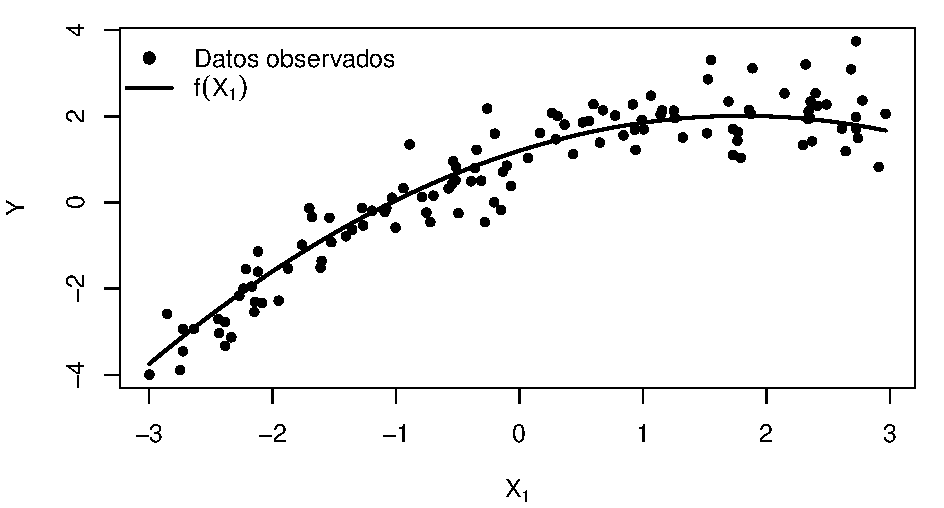
\includegraphics{1_panorama_Diapositivas-002}
\end{center}
\end{frame}

%============================================================
\begin{frame}{¿Por qué se llama ``supervisado''?}
\setkeys{Gin}{height=0.5\textheight, keepaspectratio}
\small
\textbf{Idea clave.} Al observar $Y$, el aprendizaje se puede \emph{supervisar}:
\begin{itemize}
  \item \textbf{Entrenamiento:} ajustar $f$ usando una parte de los datos.
  \item \textbf{Prueba/validación:} evaluar en datos independientes comparando
  $\hat{y}_i$ vs.\ $y_i$ con una medida de error.
\end{itemize}

\vspace{0.15cm}

\begin{center}
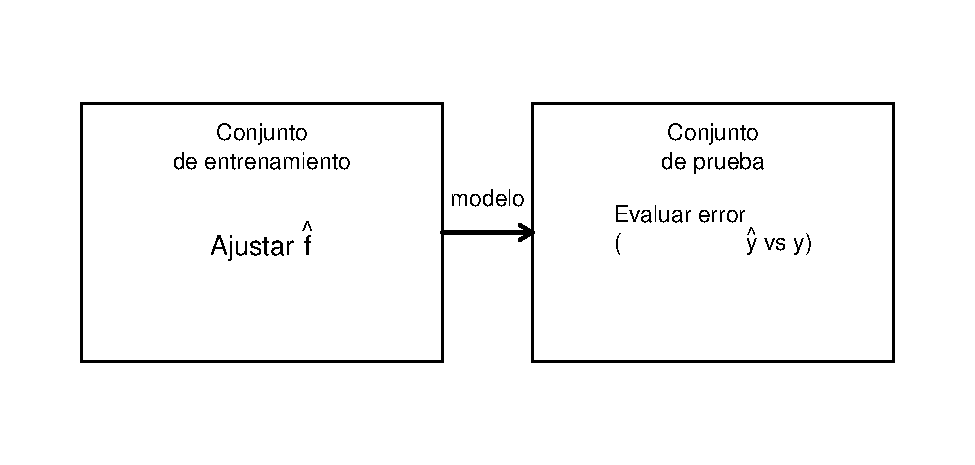
\includegraphics{1_panorama_Diapositivas-003}
\end{center}

\end{frame}

%============================================================
\begin{frame}{Métodos típicos en la categoría supervisada}
\setkeys{Gin}{height=0.5\textheight, keepaspectratio}
\small
Pertenecen a esta categoría métodos como:
\begin{itemize}
  \item \textbf{Regresión:} regresión lineal; regresión polinómica; regresión regularizada (ridge/lasso).
  \item \textbf{Clasificación:} regresión logística; árboles; k-NN; SVM; redes neuronales.
  \item \textbf{Modelos extendidos:} modelos lineales generalizados (GLM) y aditivos generalizados (GAM).
\end{itemize}

\vspace{0.1cm}

\begin{center}
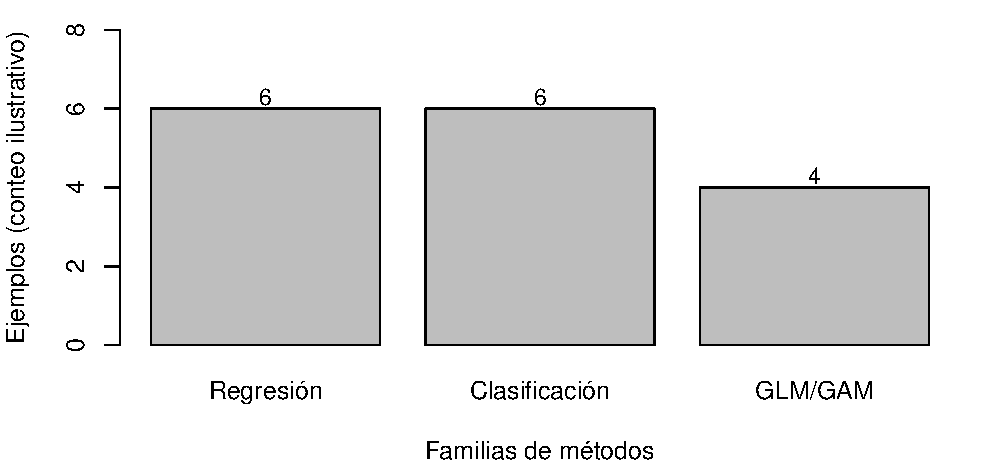
\includegraphics{1_panorama_Diapositivas-004}
\end{center}

\end{frame}
% 
%============================================================
\begin{frame}{Contraste: Aprendizaje Supervisado vs No Supervisado}
\setkeys{Gin}{height=0.4\textheight, keepaspectratio}
\small
\textbf{Idea central.}  
En el \textbf{Aprendizaje Estadístico No Supervisado} solo se observan variables
explicativas $X_1,\ldots,X_p$; no existe una variable respuesta $Y$ que permita
supervisar el aprendizaje ni evaluar el ajuste mediante un criterio externo de
error.

\begin{itemize}
  \item No hay una respuesta observable que se desee predecir.
  \item El problema no se formula en términos de predicción supervisada.
  \item La evaluación del resultado es interna al método y de carácter exploratorio.
\end{itemize}

% \vspace{0.05cm}

\begin{center}
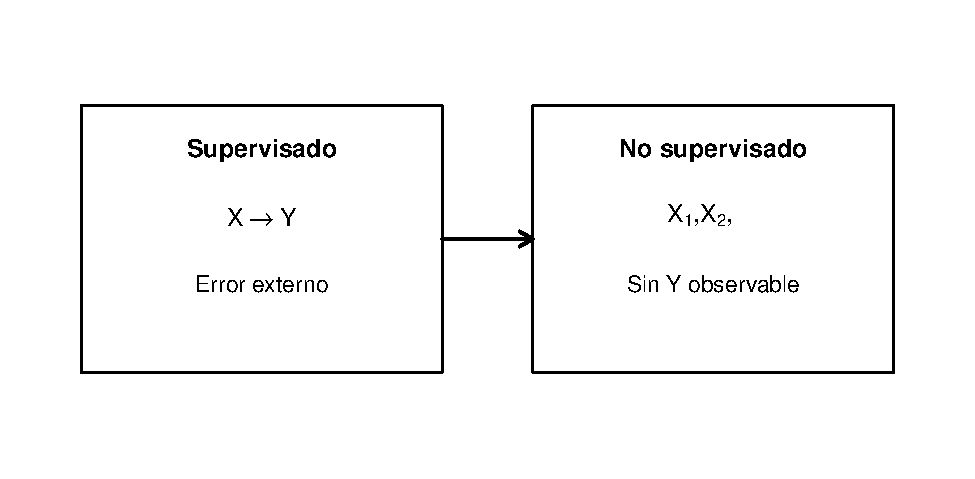
\includegraphics{1_panorama_Diapositivas-005}
\end{center}

\end{frame}

%============================================================
\begin{frame}{Objeto e interés del Análisis No Supervisado}
\setkeys{Gin}{height=0.5\textheight, keepaspectratio}
\footnotesize
En ausencia de una variable respuesta, el \textbf{análisis no supervisado} se
orienta a la \textbf{exploración de la estructura interna de los datos}.

\begin{itemize}
  \item Identificar asociaciones entre variables.
  \item Detectar similitudes o agrupamientos entre individuos.
  \item Descubrir patrones o estructuras latentes.
  \item Construir representaciones gráficas informativas.
  \item Reducir la dimensionalidad del problema.
\end{itemize}

\vspace{0.15cm}

\begin{center}
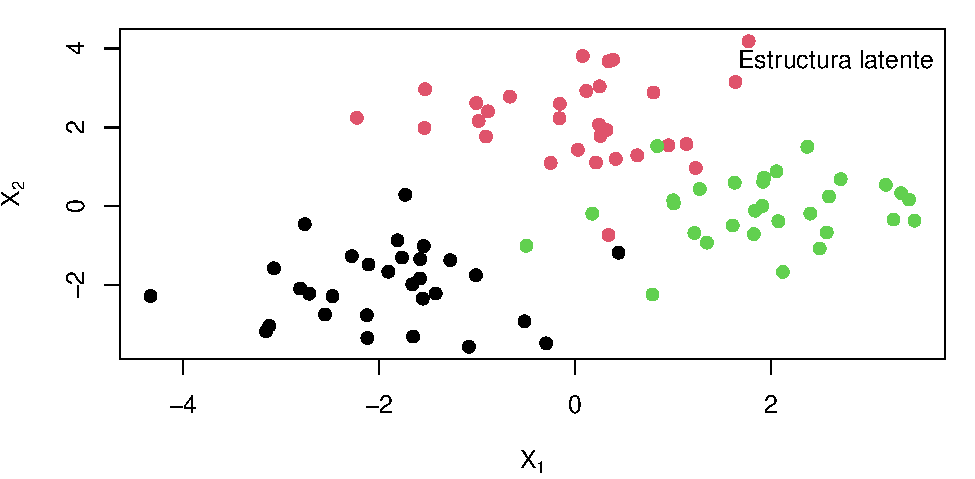
\includegraphics{1_panorama_Diapositivas-006}
\end{center}

\end{frame}
% 
%============================================================
\begin{frame}{Métodos en Aprendizaje No Supervisado}
\setkeys{Gin}{height=0.5\textheight, keepaspectratio}
\small
Como parte del \textbf{Aprendizaje Estadístico No Supervisado} se incluyen, entre otros,
los siguientes métodos:
\begin{itemize}
  \item \textbf{Reducción de dimensión:} Análisis de Componentes Principales (ACP).
  \item \textbf{Asociación en tablas categóricas:} Análisis de Correspondencias (AC) y
        Análisis de Correspondencias Múltiples (ACM).
  \item \textbf{Estructura de similitud:} métodos de agrupamiento (\emph{clustering}).
\end{itemize}

% \vspace{0.15cm}
% \textbf{Complemento sugerido.}  
% Estos métodos persiguen objetivos \emph{exploratorios}: representar la estructura interna
% de los datos mediante factores/ejes, mapas perceptuales o particiones en grupos, usando
% criterios \emph{internos} de optimalidad (inercia/varianza explicada, distancia, cohesión-separación).

% \vspace{0.15cm}

\begin{center}
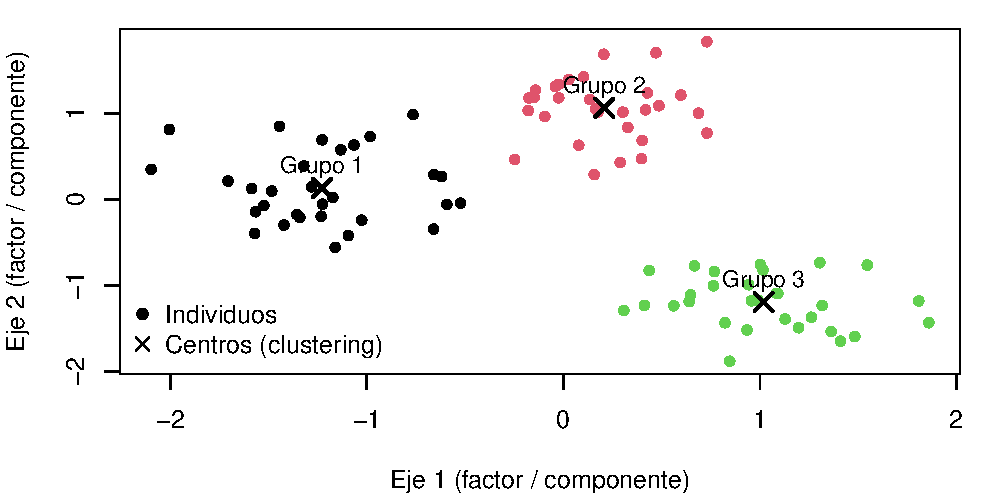
\includegraphics{1_panorama_Diapositivas-007}
\end{center}

\end{frame}

% 
\begin{frame}[fragile]{\large Mapa conceptual de métodos de aprendizaje no supervisado}

\centering
\vspace{-2mm} % opcional: sube un poco la figura

% Clave: limitar por altura (Beamer tiene poca altura útil)
\setkeys{Gin}{height=0.72\textheight, keepaspectratio}

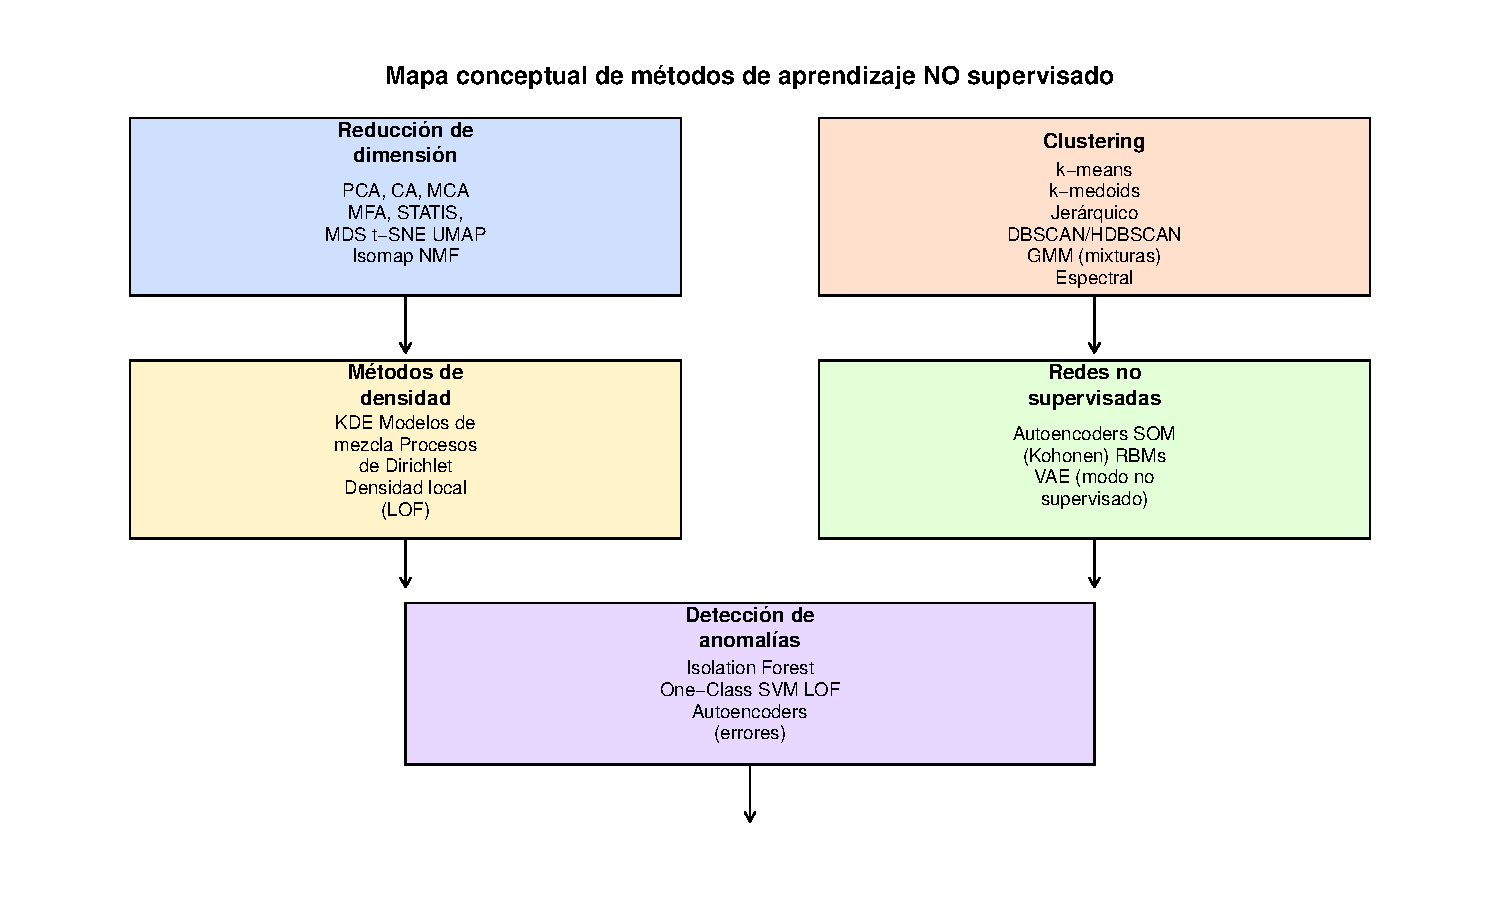
\includegraphics{1_panorama_Diapositivas-mapa_no_supervisado}
\end{frame}
% 
\begin{frame}{Métodos de reducción de las dimensiones}
\subsubsection*{Metodos basados directamente en SVD}

\begin{itemize}

  \item \textbf{PCA (Principal Components Analysis).} 
  Metodo lineal para variables numericas que busca direcciones de maxima varianza. 
  \textbf{Basado directamente en la SVD} de la matriz centrada.

  \item \textbf{CA (Correspondence Analysis).} 
  Método de análisis de dos varaibles cualitativas en tablas de contingencia basada en perfiles centrados y ponderados. 
  \textbf{Utiliza una SVD ponderada} para obtener coordenadas principales.

  \item \textbf{MCA (Multiple Correspondence Analysis).} 
  Extension del CA a multiples variables cualitativas mediante la matriz indicatoria o de Burt
  (tabla de tablas de contingencia). 
  \textbf{Fundamentado en una SVD en el espacio chi-cuadrado}.


\end{itemize}
\end{frame}
% 
\begin{frame}{Métodos de reducción de las dimensiones}
\subsubsection*{Metodos basados directamente en SVD}

\begin{itemize}


  \item \textbf{MFA (Multiple Factor Analysis).} 
  Metodo para analizar múltiples tablas en el cual unas tablas pueden ser de 
  variables cuantitativas o numéricas  y otras pueden ser de variables cualitativas
  que normaliza cada bloque y luego aplica 
  \textbf{una SVD global} para extraer factores comunes.

  \item \textbf{STATIS (incluye DiSTATIS).} 
  Metodo para tablas estructuradas en tres vias; construye una compromise matrix 
  y aplica \textbf{SVD o descomposicion espectral} para obtener configuraciones y compromisos.

  \item \textbf{MDS clasico (Classical Multidimensional Scaling o CMDS).}
  Recupera coordenadas en un espacio euclidiano mediante la 
  \textbf{descomposicion espectral de la matriz de distancias doblemente centrada}, 
  algebraicamente equivalente a una SVD.

\end{itemize}
\end{frame}
% 
\begin{frame}{Metodos no lineales o no basados en SVD}
\begin{itemize}

  \item \textbf{t-SNE (t-distributed Stochastic Neighbor Embedding).} 
  Metodo no lineal que minimiza la divergencia de Kullback--Leibler entre distribuciones de vecinos. 
  \textbf{No utiliza SVD} salvo como opcion para inicializacion.

  \item \textbf{UMAP (Uniform Manifold Approximation and Projection).} 
  Metodo de aprendizaje de variedades basado en grafos fuzzy y optimizacion de atraccion-repulsion. 
  \textbf{No utiliza SVD} excepto cuando se inicializa con PCA.

  \item \textbf{Isomap.} 
  Metodo de aprendizaje de manifolds basado en distancias geodesicas. 
  Realiza MDS al final, pero \textbf{no es un metodo basado en SVD}, 
  aunque emplea descomposicion espectral en la etapa final.

  \item \textbf{NMF (Nonnegative Matrix Factorization).} 
  Factorizacion iterativa de matrices no negativas mediante algoritmos multiplicativos o ALS. 
  \textbf{No utiliza SVD}, aunque puede inicializarse con ella.

\end{itemize}
\end{frame}
% 
\begin{frame}{Métodos de agrupamiento (Clustering)}
\begin{itemize}

  \item \textbf{K-means.} 
  Algoritmo particional que asigna cada observacion al centroide mas cercano, 
  minimizando la suma de distancias cuadraticas dentro de cada grupo. 
  Requiere fijar el numero de clusters y es sensible a valores atípicos.

  \item \textbf{K-medoids (PAM).} 
  Variante robusta de k-means que utiliza medoids (observaciones reales) en lugar de centroides, 
  adecuada para diferentes metricas de distancia y menos sensible a valores atipicos.

  \item \textbf{Clustering jerarquico (aglomerativo o divisivo).} 
  Construye un dendrograma que agrupa observaciones de manera secuencial. 
  No requiere especificar el numero de clusters a priori y permite distintos criterios de enlace 
  (single, complete, average, Ward).
\end{itemize}

\end{frame}
% 
\begin{frame}{Métodos de agrupamiento (Clustering)}
\small
\begin{itemize}

  \item \textbf{DBSCAN.} 
  Metodo basado en densidad que identifica regiones densas separadas por zonas de baja densidad. 
  Detecta ruido y produce clusters de formas arbitrarias sin necesidad de fijar el numero de grupos.

  \item \textbf{HDBSCAN.} 
  Extension jerarquica de DBSCAN que permite densidades variables. 
  Produce clusters mas estables y una mejor deteccion de ruido en datos con heterogeneidad de densidad.

  \item \textbf{GMM (Gaussian Mixture Models).} 
  Modelo probabilistico que representa los datos como una mezcla de distribuciones normales. 
  Ofrece pertenencias suaves (probabilidades) mediante el algoritmo EM y permite clusters elipticos.

  \item \textbf{Clustering espectral.} 
  Metodo que utiliza los autovectores del Laplaciano de un grafo de similitudes para representar los datos 
  en un espacio reducido, donde luego se aplica un algoritmo particional como k-means. 
  Permite detectar clusters no lineales.

\end{itemize}

\end{frame}
%
\begin{frame}{Métodos tratados en este curso}
\begin{itemize}

  \item \textbf{PCA (Principal Components Analysis).} 

  \item \textbf{CA (Correspondence Analysis).} 

  \item \textbf{MCA (Multiple Correspondence Analysis).} 

  \item \textbf{K-means.} 

  \item \textbf{Clustering jerarquico (aglomerativo o divisivo).} 

\end{itemize}
\end{frame}
% 
\begin{frame}{Elementos de álgebra lineal requeridos en análisis multivariado}

\small
\begin{itemize}
\item \textbf{Espacios vectoriales}: vectores, subespacios, bases y dimensión.
\item \textbf{Producto interno}: norma, ángulos y ortogonalidad.
\item \textbf{Proyección ortogonal} y mínimos cuadrados.
\item \textbf{Matrices}: operaciones matriciales, rango, traza e inversa (cuando existe).
\item \textbf{Matrices simétricas} y definidas positivas.
\item \textbf{Valores y vectores propios}.
\item \textbf{Teorema de la descomposición espectral (TDE)}.
\item \textbf{Teorema de la descomposición en valores singulares (TDVS)}.
\end{itemize}

\end{frame}
% 
% 
\begin{frame}{Conjuntos de datos utilizados en los ejemplos y ejercicios}
\begin{itemize}
\item \textbf{ciudades} Tabla de datos de 22 ciudades colombianas con 6 variables referentes a la educación y número de habitantes.

\item etiq\_ciudades

\item \textbf{ciudadesC} Tabla de datos de 22 ciudades colombianas con 84 variables clasificadas en grupos que abarcan temas como Recursos Humanos, Ciencia y Tecnología, Infraestructura, Finazas públicas entre otros.

\item \textbf{Etiquetas ciudades} Contiene las etiquetas del archivo ciudadesC

\item \textbf{ARWU\_100\_top} Tabla de datos de puntajes y posiciones de las 100 mejores universidades del mundo según el ranking Academic Rank of World Universities (ARWU)

\item arwu

\item \textbf{r14\_Sci\_Qs\_Webometrics} Tabla de datos de puntajes y posiciones de 149 universidades latinoamericanas según estos tres rankings

\item confianza Tabla con lresultados sobre confianza en instituciones

\item ConfianzaJUsticia. Tabla resultados de confianza en la justicia

\item RankLatino Rankins latinoamericanos

\item CCLatin Ciudades latinoamericanas

\item rankings Rankings 

\end{itemize}
\end{frame}
% 
\begin{frame}{\centering \textcolor{yellow}{Panorama del análisis multivariado}}
{\large Tipos de variables para visualización de datos}

En visualización y análisis no supervisado, las variables se clasifican
según el \textbf{tipo de información que contienen}:
\begin{itemize}

\item Esta clasificación determina:
  \begin{itemize}
  \item los métodos gráficos apropiados,
  \item las métricas de similitud o distancia,
  \item y las técnicas multivariadas aplicables.
  \end{itemize}
\item Distinguimos principalmente entre:
  \begin{itemize}
  \item \textbf{variables cualitativas o categóricas},
  \item \textbf{variables cuantitativas o numéricas}.
  \end{itemize}
\end{itemize}

\end{frame}
% 
\begin{frame}{Variables cualitativas}

\begin{itemize}
\item Describen \textbf{cualidades, categorías o clases} de los objetos.
\item No admiten operaciones aritméticas directas.
\item Se distinguen dos tipos principales:
  \begin{itemize}
  \item \textbf{Nominales}: 
    \begin{itemize}
    \item funcionan como códigos sin orden implícito,
    \item ejemplos: ciudades, países, identificadores.
    \end{itemize}
  \item \textbf{Categóricas (u ordinales)}:
    \begin{itemize}
    \item representan categorías con \textbf{orden o jerarquía},
    \item ejemplos: niveles educativos, estratos socioeconómicos,
    posiciones en rankings universitarios.
    \end{itemize}
  \end{itemize}
\item Sus valores se denominan \textbf{modalidades} u \textbf{opciones de respuesta}.
\end{itemize}

\end{frame}
% 
\begin{frame}{Variables cuantitativas}

\begin{itemize}
\item Se expresan en una \textbf{escala numérica} y admiten comparaciones métricas.
\item Permiten definir distancias y aplicar operaciones aritméticas.
\item Se dividen en:
  \begin{itemize}
  \item \textbf{Continuas}:
    \begin{itemize}
    \item toman valores en un intervalo continuo,
    \item interpretación directa,
    \item ejemplos: altura, edad, ingresos, longitud.
    \end{itemize}
  \item \textbf{Discretas}:
    \begin{itemize}
    \item toman valores enteros,
    \item ejemplos: número de habitantes, conteos de eventos,
    \item promedios pueden producir valores no directamente interpretables
    (p.\ ej., 4.6 aviones por minuto).
    \end{itemize}
  \end{itemize}
\end{itemize}

\end{frame}
% 
\begin{frame}{Tipos de variables y métodos multivariados}

\begin{itemize}
\item La elección del método de análisis multivariado depende
directamente del \textbf{tipo de variables} disponibles.
\item En análisis no supervisado, los métodos más utilizados son:
\end{itemize}

\vspace{2mm}

\begin{block}{Correspondencia entre variables y métodos}
\begin{itemize}
\item \textbf{PCA (Análisis de Componentes Principales)}  
Variables \textbf{cuantitativas} (continuas o discretas tratadas como numéricas).

\item \textbf{MCA (Análisis de Correspondencias Múltiples)}  
Variables \textbf{cualitativas} (nominales u ordinales codificadas en modalidades).

\item \textbf{MFA (Análisis Factorial Múltiple)}  
Conjuntos de variables \textbf{mixtas} o \textbf{estructuradas en grupos}
(cuantitativas y/o cualitativas).
\end{itemize}
\end{block}

\vspace{0.5mm}
\centering
\textcolor{blue}{{\small \textit{El tipo de variable determina la geometría del espacio y la métrica utilizada.}}}

\end{frame}

% 
\begin{frame}{Motivación: El papel de las componentes principales}

\begin{itemize}
\item Los \textbf{gráficos de dispersión} permiten explorar relaciones entre pares de
variables cuantitativas e identificar patrones, tendencias y valores atípicos.
\item Mediante colores, tamaños o etiquetas es posible incorporar información adicional,
pero la representación sigue estando \textbf{limitada a dos dimensiones}.
\item Cuando el número de variables es grande, los planos definidos por variables
originales \textbf{no capturan adecuadamente} la estructura global de los datos.
\item Las \textbf{componentes principales} definen nuevos ejes, como combinaciones
lineales de las variables originales, que \textbf{maximizan la variabilidad}.
\item Los planos generados por las primeras componentes proporcionan
\textbf{representaciones más informativas y sintéticas} de los datos.
\end{itemize}

\end{frame}
% 
\begin{frame}[fragile]{Motivación: variables originales vs plano PCA}

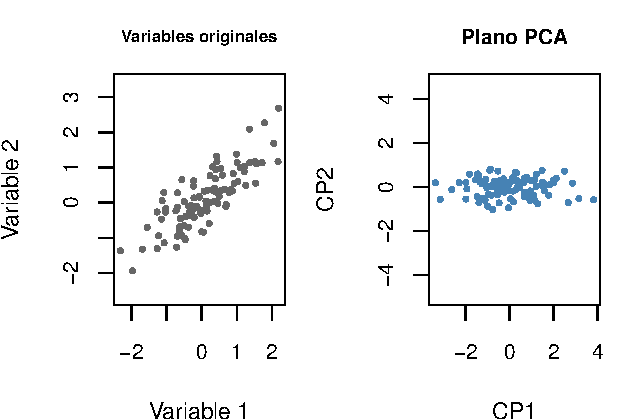
\includegraphics{1_panorama_Diapositivas-scatter_vs_pca}
\end{frame}
% 
\begin{frame}{Rankings universitarios}

\begin{ejem}


\begin{itemize}
  \item Los \textbf{rankings universitarios} son clasificaciones basadas en criterios definidos por las entidades que los elaboran.
  \item Dichos criterios responden a un \textbf{modelo implícito de universidad de élite}, que puede variar entre rankings.
  \item Por esta razón, los resultados y ponderaciones \textbf{difieren significativamente} de un ranking a otro.
  \item Entre los criterios más frecuentes se encuentran:
  \begin{itemize}
    \item producción e impacto de publicaciones científicas,
    \item calidad e impacto de las revistas,
    \item actividades de investigación e innovación,
    \item proporción de docentes con doctorado,
    \item reputación académica y entre empleadores,
    \item presencia e internacionalización,
    \item premios de docentes y egresados.
  \end{itemize}
\end{itemize}
\end{ejem}

\end{frame}
% 
\begin{frame}{Rankings universitarios}

\begin{ejem}


\begin{itemize}
\item Desde el punto de vista estadístico, los rankings universitarios se construyen
a partir de \textbf{múltiples indicadores} asociados a diferentes criterios.
\item Los indicadores suelen ser \textbf{normalizados o estandarizados} para hacerlos comparables.
\item Luego se calcula un \textbf{puntaje total} mediante una \textbf{suma ponderada}
(combinación lineal ponderada) de los indicadores; los pesos reflejan el
\textbf{modelo implícito de universidad} del ranking.
\item Con el puntaje total se obtiene un \textbf{ordenamiento}: puesto 1 al mayor puntaje,
puesto 2 al siguiente, etc.
\item El resultado es un \textbf{orden relativo}; las diferencias numéricas entre puntajes
no necesariamente tienen interpretación como “distancias”.
\end{itemize}
\end{ejem}

\end{frame}
% 
\begin{frame}{ARWU Cont.}

\begin{ejem}
\footnotesize 


\begin{itemize}
\item Uno de los rankings más reconocidos y selectivos es el
\textbf{Academic Ranking of World Universities (ARWU)}.
\item Su metodología se basa en indicadores asociados principalmente al desempeño
académico y de investigación, entre ellos:
  \begin{itemize}
  \item \textbf{Premios Nobel y Medallas Fields} de egresados (Alumni) y docentes (Staff),
  \item \textbf{investigadores altamente citados} (Highly Cited Researchers),
  \item \textbf{publicaciones en \emph{Nature} y \emph{Science}},
  \item \textbf{artículos indexados} en índices bibliométricos (p.\ ej., SCIE/SSCI),
  \item \textbf{desempeño per cápita} del personal académico (PCP).
  \end{itemize}
\item En este ejemplo se consideran las universidades ubicadas en los \textbf{100 primeros puestos}
del ARWU (año 2013) y se analizan sus posiciones \textbf{mundial} y, por derivación,
sus posiciones \textbf{nacional} y \textbf{regional}. 
\item Para más detalles metodológicos, ver \cite{liu2005academic}.
\end{itemize}

\end{ejem}

\end{frame}
% 
% 
% 
\begin{frame}[fragile]{ARWU Cont.}

\begin{ejem}
\textbf{Distribución por país en el Top 100 (ARWU 2013)}\\[1mm]

%---------------- Tabla ----------------
\begin{table}[!h]
\centering\begingroup\fontsize{6}{8}\selectfont

\resizebox{\ifdim\width>\linewidth\linewidth\else\width\fi}{!}{
\begin{tabular}{rrrrrrrrrrrrrrrr}
\toprule
US & UK & GE & JP & CA & AS & FR & SE & SW & DE & NL & BE & FI & IR & NW & RU\\
\midrule
54 & 11 & 5 & 5 & 4 & 3 & 3 & 3 & 3 & 2 & 2 & 1 & 1 & 1 & 1 & 1\\
\bottomrule
\end{tabular}}
\endgroup{}
\end{table}
\vspace{1mm}

%---------------- Texto ----------------
{\footnotesize
En la Tabla \ref{tab:TablARWUpais} se muestra la distribución del número de
universidades por país entre las \textbf{100 primeras} del ARWU 2013.
Se observa una alta concentración en pocos países: \textbf{Estados Unidos (US)}
aporta \textbf{54} universidades, seguido por el \textbf{Reino Unido (UK)} con
\textbf{11}. En un segundo nivel aparecen \textbf{Alemania (GE)} y
\textbf{Japón (JP)} con \textbf{5} universidades cada uno.
}

\end{ejem}

\end{frame}

\begin{frame}{ARWU Cont.}

\setlength{\abovecaptionskip}{2pt}  % <-- reduce espacio arriba del caption
\setlength{\belowcaptionskip}{1pt}  % <-- reduce espacio debajo del caption
\begin{table}[!h]
\centering
\caption{\label{tab: TablARWU}20 mejores universidades del mundo según el ARWU 2013}
\centering
\resizebox{\ifdim\width>\linewidth\linewidth\else\width\fi}{!}{
\begin{tabular}[t]{lllrrr}
\toprule
Institution & Region & Country & Regional.Rank & World.Rank & National.Rank\\
\midrule
\cellcolor{gray!10}{Harvard University} & \cellcolor{gray!10}{Americas} & \cellcolor{gray!10}{US} & \cellcolor{gray!10}{1} & \cellcolor{gray!10}{1} & \cellcolor{gray!10}{1}\\
University of California, Berkeley & Americas & US & 2 & 2 & 2\\
\cellcolor{gray!10}{Stanford University} & \cellcolor{gray!10}{Americas} & \cellcolor{gray!10}{US} & \cellcolor{gray!10}{3} & \cellcolor{gray!10}{3} & \cellcolor{gray!10}{3}\\
Massachusetts Institute of Technology (MIT) & Americas & US & 4 & 4 & 4\\
\cellcolor{gray!10}{University of Cambridge} & \cellcolor{gray!10}{Europe} & \cellcolor{gray!10}{UK} & \cellcolor{gray!10}{1} & \cellcolor{gray!10}{5} & \cellcolor{gray!10}{1}\\
\addlinespace
California Institute of Technology & Americas & US & 5 & 6 & 5\\
\cellcolor{gray!10}{Princeton University} & \cellcolor{gray!10}{Americas} & \cellcolor{gray!10}{US} & \cellcolor{gray!10}{6} & \cellcolor{gray!10}{7} & \cellcolor{gray!10}{6}\\
Columbia University & Americas & US & 7 & 8 & 7\\
\cellcolor{gray!10}{University of Chicago} & \cellcolor{gray!10}{Americas} & \cellcolor{gray!10}{US} & \cellcolor{gray!10}{8} & \cellcolor{gray!10}{9} & \cellcolor{gray!10}{8}\\
University of Oxford & Europe & UK & 2 & 10 & 2\\
\addlinespace
\cellcolor{gray!10}{Yale University} & \cellcolor{gray!10}{Americas} & \cellcolor{gray!10}{US} & \cellcolor{gray!10}{9} & \cellcolor{gray!10}{11} & \cellcolor{gray!10}{9}\\
Cornell University & Americas & US & 10 & 12 & 10\\
\cellcolor{gray!10}{University of California, Los Angeles} & \cellcolor{gray!10}{Americas} & \cellcolor{gray!10}{US} & \cellcolor{gray!10}{11} & \cellcolor{gray!10}{13} & \cellcolor{gray!10}{11}\\
University of California, San Diego & Americas & US & 12 & 14 & 12\\
\cellcolor{gray!10}{University of Pennsylvania} & \cellcolor{gray!10}{Americas} & \cellcolor{gray!10}{US} & \cellcolor{gray!10}{13} & \cellcolor{gray!10}{15} & \cellcolor{gray!10}{13}\\
\addlinespace
University of Washington & Americas & US & 14 & 16 & 14\\
\cellcolor{gray!10}{University of Wisconsin - Madison} & \cellcolor{gray!10}{Americas} & \cellcolor{gray!10}{US} & \cellcolor{gray!10}{15} & \cellcolor{gray!10}{17} & \cellcolor{gray!10}{15}\\
The Johns Hopkins University & Americas & US & 16 & 18 & 16\\
\cellcolor{gray!10}{University of California, San Francisco} & \cellcolor{gray!10}{Americas} & \cellcolor{gray!10}{US} & \cellcolor{gray!10}{16} & \cellcolor{gray!10}{18} & \cellcolor{gray!10}{17}\\
The University of Tokyo & Asia/Pacific & JP & 1 & 20 & 1\\
\bottomrule
\end{tabular}}
\end{table}
\end{frame}
% 
\begin{frame}{ARWU Cont.}
\setkeys{Gin}{width=0.7\textwidth, height=0.5\textheight,keepaspectratio} % para redefinir el tamaño de los graficos
\begin{figure}[H]
\captionsetup[subfigure]{font=tiny}
\captionsetup{font=footnotesize}


% \centering
\captionsetup[subfigure]{justification=centering}

\begin{subfigure}[t]{0.48\textwidth}
\centering
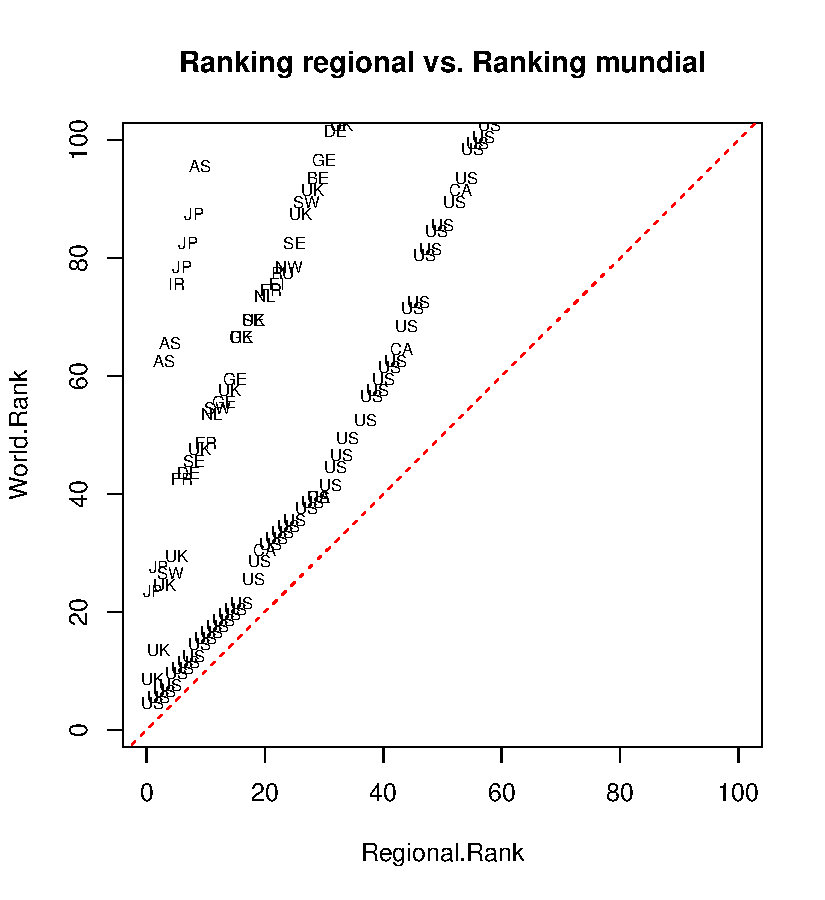
\includegraphics{1_panorama_Diapositivas-fig_arwu_left}
\caption{Posición regional vs. posición mundial de las primeras 100 universidades según el ranking ARWU, etiquetadas por su país de origen.}
\label{arwuRegMunPaises}
\end{subfigure}
\hfill
\begin{subfigure}[t]{0.48\textwidth}
% \centering
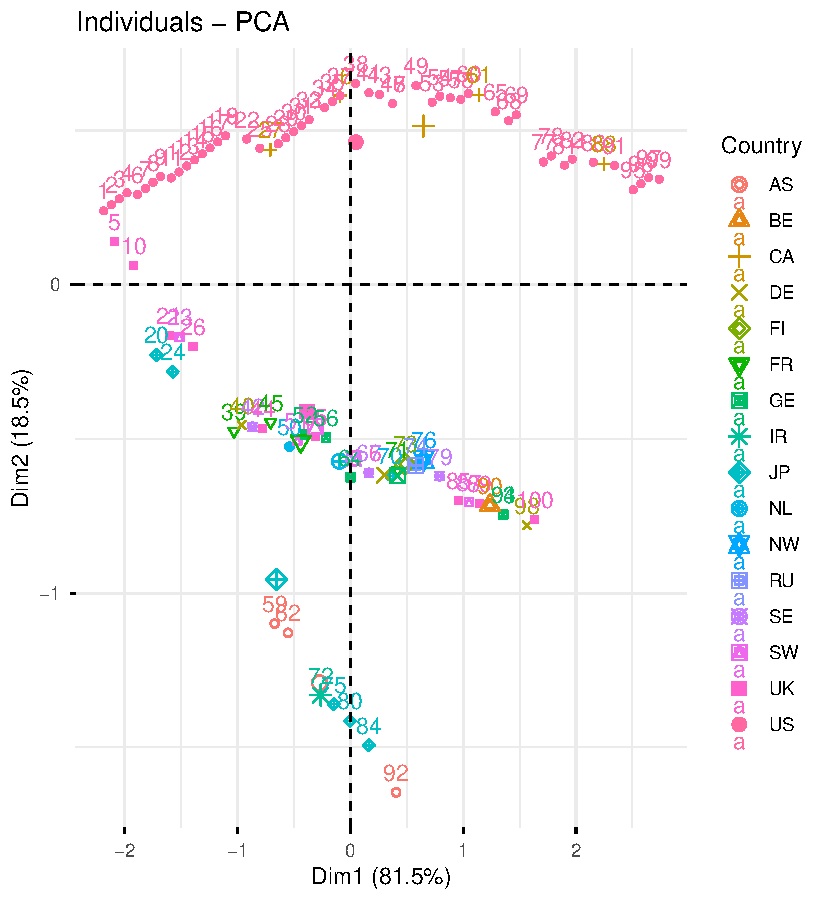
\includegraphics{1_panorama_Diapositivas-fig_arwu_right}
\caption{Posición regional vs. posición mundial de las primeras 100 universidades según el ranking ARWU, sobre las dos primeras componentes principales.}
\label{arwuRegMunPaisesacp}
\end{subfigure}
\caption{Comparación de la visualización de los datos originales con su proyección sobre las dos primeras componetes principales}
\end{figure}
\end{frame}
% 

% 
\begin{frame}{Rankings universidades latinoamericanas}
\begin{ejem}

\textbf{Scimago}
\small 
\vspace{1mm}

\textbf{Sobre inconsistencias en algunos rankings universitarios}

\vspace{1mm}

Scimago es un ranking orientado a la evaluación de la
\textbf{actividad investigativa} de universidades e instituciones de investigación.
Su metodología incluye nueve indicadores de investigación, entre los que se
encuentran medidas de impacto, productividad, colaboración internacional,
publicaciones de alta calidad, liderazgo científico, excelencia y talento
científico, además de tres indicadores de innovación y tres de factor social.
Por su enfoque, este ranking privilegia el desempeño científico medido a partir
de la producción y el impacto de la investigación.
Para más detalles, véase \cite{scimagoi}.
\end{ejem}
\end{frame}
% 
\begin{frame}{Rankings universidades latinoamericanas}
\begin{ejem}

\textbf{Webranking}
\small
\vspace{1mm}

\textbf{Sobre inconsistencias en algunos rankings universitarios}

\vspace{1mm}

El Webranking es un ranking de \textbf{presencia en la web} que evalúa la visibilidad
institucional de las universidades a partir de indicadores como el número de
enlaces entrantes al dominio institucional, el número de páginas web y la cantidad
de archivos publicados en formatos \texttt{pdf}, \texttt{doc}, \texttt{xls}, entre otros,
alojados en los dominios universitarios. Adicionalmente, incorpora un indicador
de excelencia tomado del ranking Scimago.
Este enfoque prioriza la visibilidad digital y la difusión de contenidos académicos
en la web. Para más detalles, véase \cite{webR}.

\end{ejem}
\end{frame}
% 
\begin{frame}{Rankings universidades latinoamericanas}
\begin{ejem}

\textbf{QS}
\small
\vspace{1mm}

\textbf{Sobre inconsistencias en algunos rankings universitarios}

\vspace{1mm}

El ranking QS combina indicadores de \textbf{reputación} y desempeño académico.
Incluye dos indicadores de reputación —uno medido entre pares académicos y otro
entre empleadores— obtenidos mediante encuestas, así como la razón
estudiantes/profesor, el número de profesores con doctorado, el número de citas
por artículo, el promedio de artículos por docente y un indicador de impacto web
tomado del Webranking. Los indicadores de reputación tienen una ponderación del
\textbf{25\%} cada uno, mientras que los restantes indicadores tienen una
ponderación del \textbf{10\%} cada uno.
Por esta razón, este ranking se considera principalmente un ranking de
\textbf{reputación universitaria}. Para detalles metodológicos (2014), véase
\cite{QsRank}.

\end{ejem}
\end{frame}


\begin{frame}{Rankings universidades latinoamericanas}

\begin{ejem}
\begin{table}[!h]
\centering
\caption{\label{tab:TablaRankLatinos}Primeras 20 universidades según el ranking Qs}
\centering
\resizebox{\ifdim\width>\linewidth\linewidth\else\width\fi}{!}{
\begin{tabular}[t]{lllrrr}
\toprule
  & UniPais & Pais & SC.Lac.Ranking & QS.Ranking & WEB.Ranking.LA\\
\midrule
\cellcolor{gray!10}{10} & \cellcolor{gray!10}{POTFIC CATOLICA DE  - CHL} & \cellcolor{gray!10}{CHL} & \cellcolor{gray!10}{13} & \cellcolor{gray!10}{1} & \cellcolor{gray!10}{24}\\
1 & DE SAO PAULO (USP) - BRA & BRA & 1 & 2 & 1\\
\cellcolor{gray!10}{3} & \cellcolor{gray!10}{Es DE CAMPIS (UNICAMP) - BRA} & \cellcolor{gray!10}{BRA} & \cellcolor{gray!10}{4} & \cellcolor{gray!10}{3} & \cellcolor{gray!10}{8}\\
5 & DO RD Janeiro FED - BRA & BRA & 5 & 4 & 5\\
\cellcolor{gray!10}{21} & \cellcolor{gray!10}{LOS ANDES  - COL} & \cellcolor{gray!10}{COL} & \cellcolor{gray!10}{47} & \cellcolor{gray!10}{5} & \cellcolor{gray!10}{38}\\
\addlinespace
9 & U de  - CHL & CHL & 10 & 6 & 6\\
\cellcolor{gray!10}{61} & \cellcolor{gray!10}{TECNOLOGICO DE MONTERREY (ITESM) - MEX} & \cellcolor{gray!10}{MEX} & \cellcolor{gray!10}{56} & \cellcolor{gray!10}{7} & \cellcolor{gray!10}{28}\\
2 & NAL AUTONO DE  (UM) - MEX & MEX & 2 & 8 & 2\\
\cellcolor{gray!10}{6} & \cellcolor{gray!10}{EEs PAULISTA JULIO MESQU  - BRA} & \cellcolor{gray!10}{BRA} & \cellcolor{gray!10}{3} & \cellcolor{gray!10}{9} & \cellcolor{gray!10}{11}\\
7 & Fe DO RG D SUL - BRA & BRA & 6 & 10 & 3\\
\addlinespace
\cellcolor{gray!10}{8} & \cellcolor{gray!10}{Fe MG - BRA} & \cellcolor{gray!10}{BRA} & \cellcolor{gray!10}{8} & \cellcolor{gray!10}{10} & \cellcolor{gray!10}{9}\\
20 & CONCEPCION - CHL & CHL & 28 & 12 & 32\\
\cellcolor{gray!10}{37} & \cellcolor{gray!10}{POTFIC CATOLICA DO R de Janeiro -PUC - BRA} & \cellcolor{gray!10}{BRA} & \cellcolor{gray!10}{40} & \cellcolor{gray!10}{13} & \cellcolor{gray!10}{30}\\
26 & NAL DE  - COL & COL & 18 & 14 & 10\\
\cellcolor{gray!10}{11} & \cellcolor{gray!10}{Fe DE SAO PAULO (UNIFESP) - BRA} & \cellcolor{gray!10}{BRA} & \cellcolor{gray!10}{9} & \cellcolor{gray!10}{15} & \cellcolor{gray!10}{54}\\
\addlinespace
42 & SANTIAGO DE  (USACH) - CHL & CHL & 60 & 16 & 34\\
\cellcolor{gray!10}{15} & \cellcolor{gray!10}{DE BRASILIA - BRA} & \cellcolor{gray!10}{BRA} & \cellcolor{gray!10}{19} & \cellcolor{gray!10}{17} & \cellcolor{gray!10}{13}\\
16 & Fe DE SAO CARLOS - BRA & BRA & 21 & 18 & 43\\
\cellcolor{gray!10}{4} & \cellcolor{gray!10}{BUENOS AIRES - ARG} & \cellcolor{gray!10}{ARG} & \cellcolor{gray!10}{7} & \cellcolor{gray!10}{19} & \cellcolor{gray!10}{7}\\
116 & AUSTRAL - ARG & ARG & 250 & 20 & 262\\
\bottomrule
\end{tabular}}
\end{table}
\end{ejem}

\end{frame}
% 
\begin{frame}{Rankings universidades latinoamericanas}

\begin{ejem}
\setkeys{Gin}{width=0.7\textwidth, height=0.5\textheight,keepaspectratio} % para redefinir el tamaño de los graficos
\begin{figure}[H]
	\centering
	
% ====================== nueva versión===========================
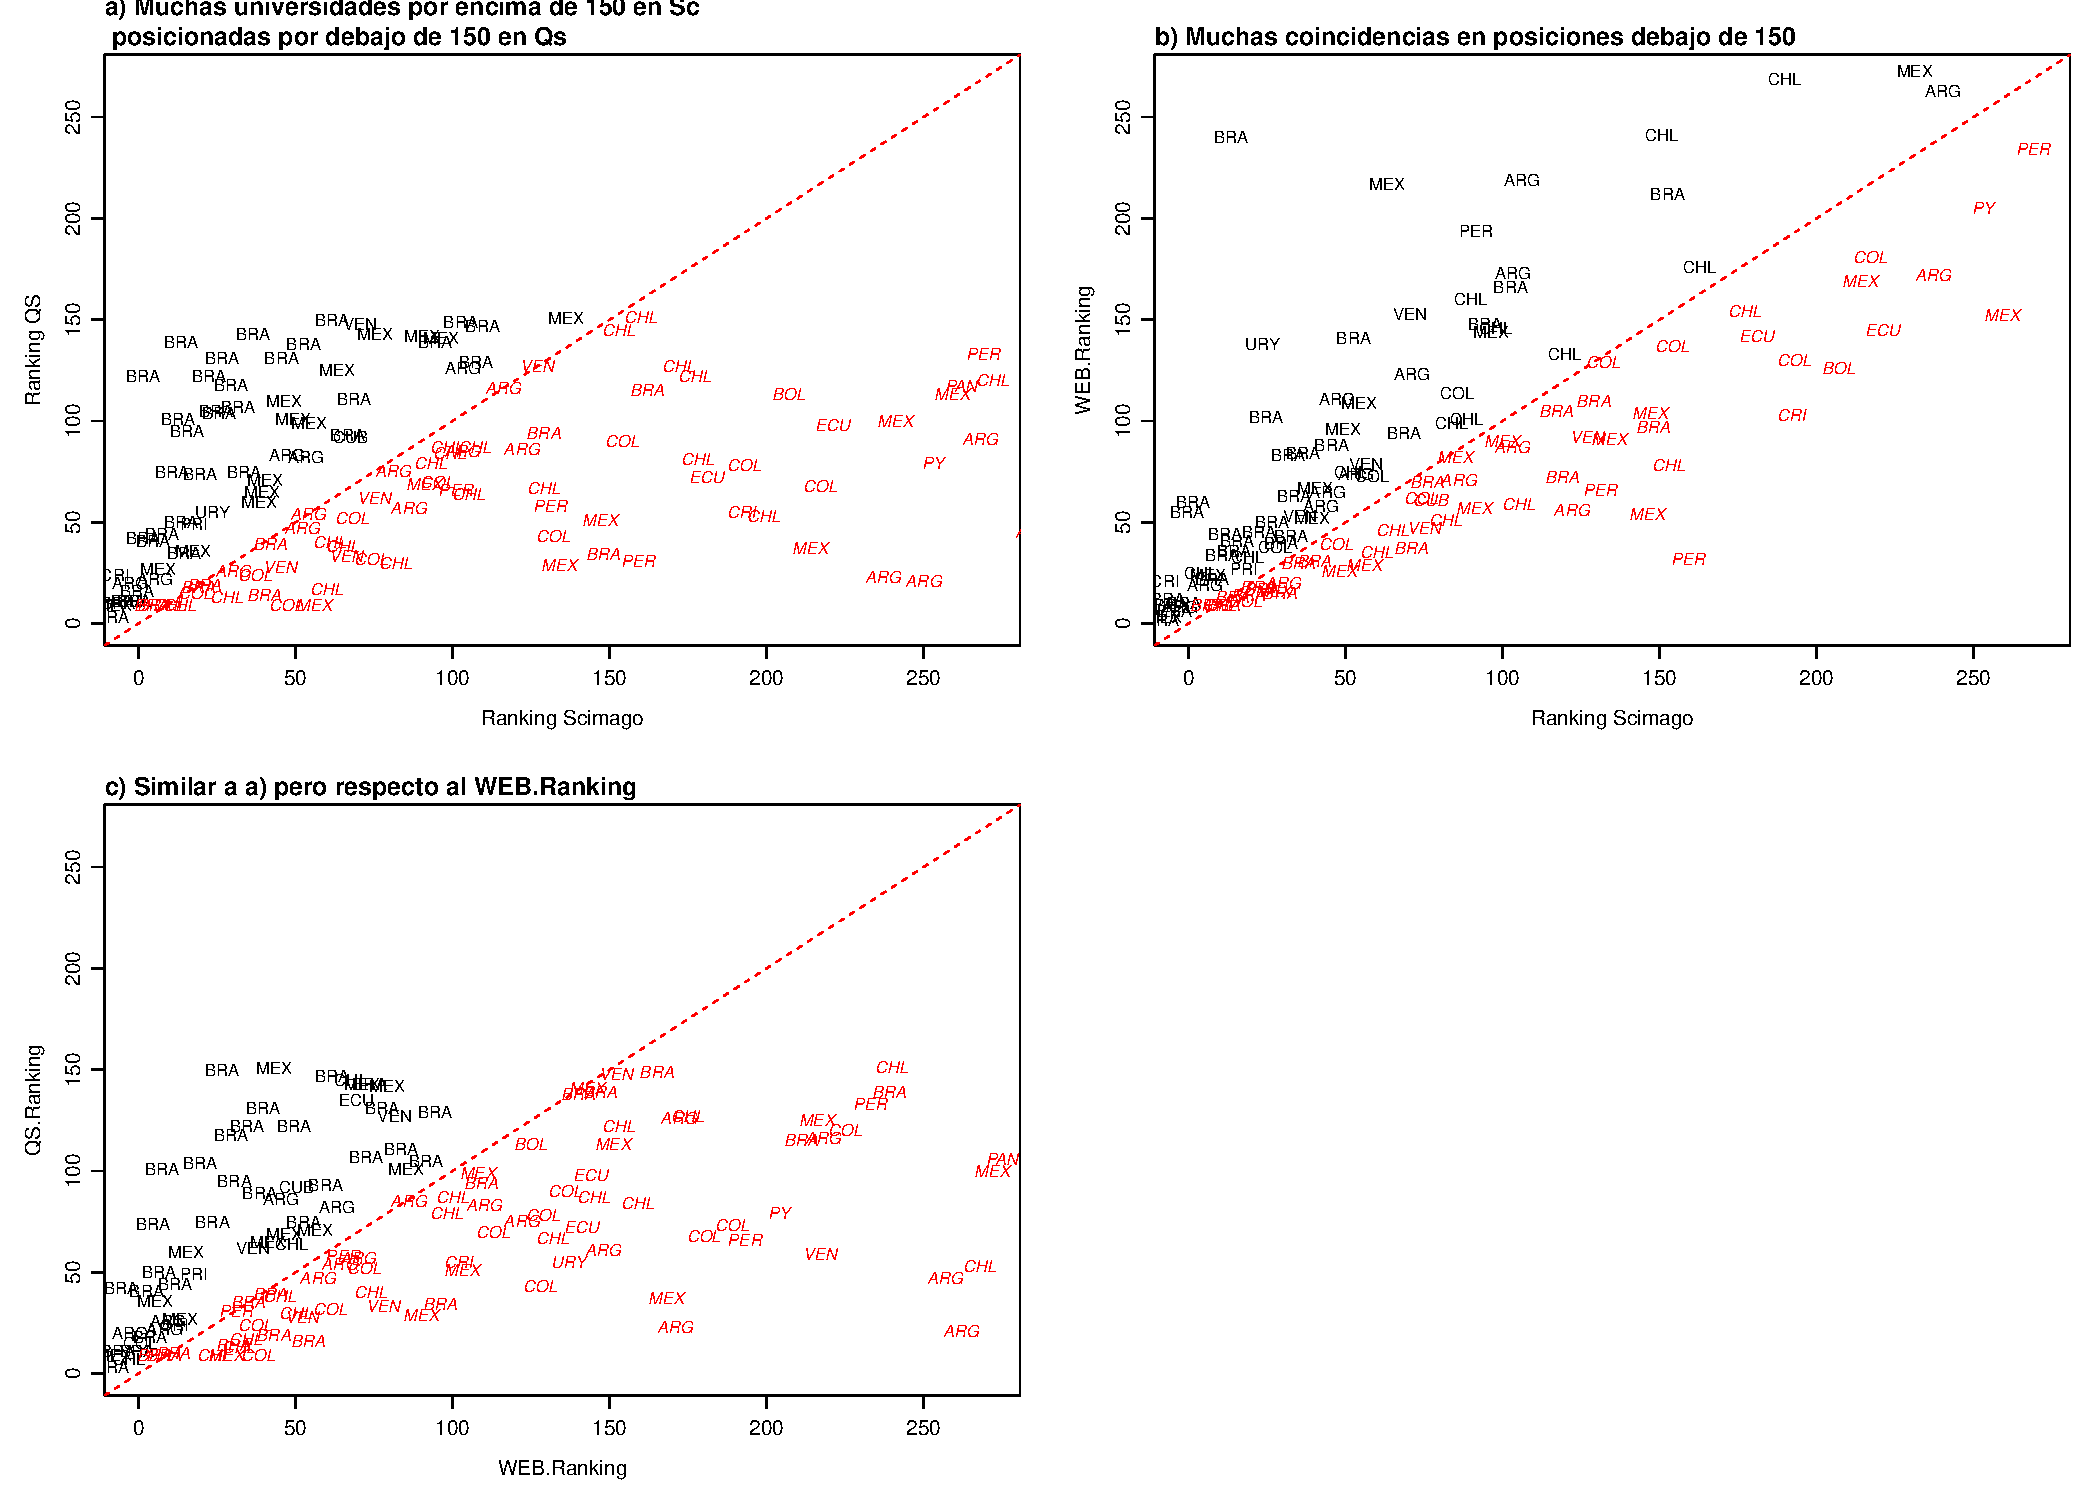
\includegraphics{1_panorama_Diapositivas-fig_grid_rankings}
\caption{Comparación entre rankings (Scimago, QS y WEB). Entre más lejos de la diagonal mas diferentes son los rankings correspondientes}
\label{fig:grid_rankings}
\end{figure}
\end{ejem}

\end{frame}
% 
\begin{frame}{Rankings universidades latinoamericanas}
\footnotesize
\begin{ejem}
\setkeys{Gin}{width=0.7\textwidth, height=0.5\textheight,keepaspectratio} % para redefinir el tamaño de los graficos
\setlength{\abovecaptionskip}{2pt}  % <-- reduce espacio arriba del caption
\setlength{\belowcaptionskip}{1pt}  % <-- reduce espacio debajo del caption

\begin{figure}[H]
	\centering

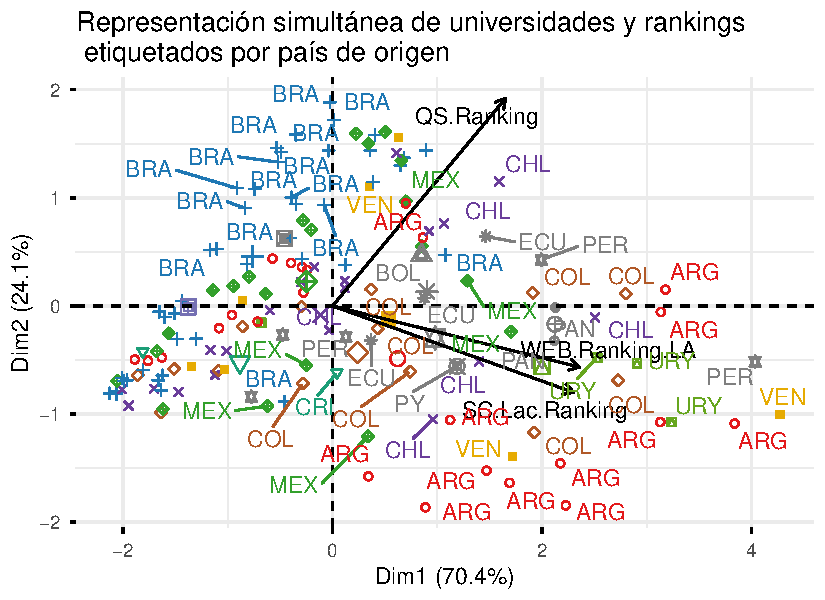
\includegraphics{1_panorama_Diapositivas-016}
\caption{Los dos vectores que representan los ranking SC.Lac.Ranking y WEB.Ranking.LA reflejan su grado de asociación visualizado en la gráfica \ref{fig:grid_rankings} b). El vector QS.Ranking muestra el grado de independencia de éste con los otros dos rankings, ya identificada en los gráficos \ref{fig:grid_rankings} a) y \ref{fig:grid_rankings} c).}
\label{fig:acp_rankings}
\end{figure}
\end{ejem}

\end{frame}
% 
\begin{frame}{Correspondencias simples y análisis de tablas de contingencia \textcolor{magenta}{(EMV)}}

Una \textbf{tabla de contingencia} es un arreglo de las frecuencias de ocurrencia simultánea de las opciones de respuesta de dos variables cualitativas, $X$ con $I$ modalidades en las filas y $Y$ con $J$ modalidades en las columnas. Formalmente se escribe como

\[
G=\{n_{ij}\}=
\left(
\begin{array}{cccc}
n_{11}& n_{12}& \cdots& n_{1J}\\
n_{21}& n_{22}& \cdots& n_{2J}\\
\vdots& \vdots& \ddots& \vdots\\
n_{I1}& n_{I2}& \cdots& n_{IJ}
\end{array}
\right),
\]

donde $n_{ij}$ representa el número de individuos que simultáneamente presentan la modalidad $i$ de $X$ y la modalidad $j$ de $Y$. El tamaño muestral total es

\[
n=\sum_{i=1}^{I}\sum_{j=1}^{J} n_{ij}.
\]

\end{frame}
% 
\begin{frame}{Perfiles fila y perfiles columna}

El análisis de una tabla de contingencia permite estudiar la 
\textbf{asociación entre variables cualitativas}. El análisis se hace por medio de los perfiles fila y columna 

Cada fila de la tabla puede interpretarse como un \textbf{perfil fila}, es decir,
una distribución condicional de $Y$ dada la modalidad $i$ de $X$:

\[
f_{ij}=\frac{n_{ij}}{n_{i\cdot}},\quad \text{donde}\, n_{i\cdot}=\sum_{j=1}^J n_{ij}
\qquad j=1,\ldots,J.
\]

Análogamente, cada columna define un \textbf{perfil columna}, correspondiente a
la distribución condicional de $X$ dada la modalidad $j$ de $Y$:

\[
c_{ij}=\frac{n_{ij}}{n_{\cdot j}}, \text{donde}\quad n_{\cdot j}=\sum_{i=1}^I n_{ij}.
\qquad i=1,\ldots,I.
\]

\end{frame}
% 
\begin{frame}{Conexión con la teoría de probabilidad}
En el contexto de teoría de probabilidad, si dos variables aleatorias $X$ y $Y$ son independientes, entonces:
$$P(X=i,Y=j) = P(X=i)P(Y=j), \quad i=1,\ldots, I, \, j=1,\ldots, J  $$
Empíricamente, esta relación de independencia entre $X$ y $Y$ se traduce en que aproximadamente.

$$
\frac{n_{ij}}{n} \approx \frac{n_{i\cdot}}{n}\frac{n_{\cdot j}}{n},
$$
entonces las desviaciones respecto a esta estructura de independencia contienen toda la información sobre la asociación entre modalidades.
\end{frame}
% 
\begin{frame}{Distancia Chi-cuadrado}
Para cuantificar la proximidad entre perfiles se introduce naturalmente la \textbf{distancia $\chi^2$}. Entre dos perfiles fila $i$ y $i'$ se define como

$$
d_{\chi^2}^2(i,i')=
\sum_{j=1}^J
\frac{1}{n_{\cdot j}/n}
\left(
\frac{n_{ij}}{n_{i\cdot}}-
\frac{n_{i'j}}{n_{i'\cdot}}
\right)^2.
$$

Análogamente, puede definirse una distancia $\chi^2$ entre perfiles columna.

Esta métrica pondera las diferencias entre perfiles según la importancia de cada modalidad, medida por su frecuencia marginal, y constituye el fundamento geométrico del \textbf{Análisis de Correspondencias Simples}, que busca representar estas nubes de perfiles en espacios de baja dimensión conservando, en lo posible, dichas distancias.
\end{frame}

\begin{frame}{Correspondencias simples y análisis de tablas de contingencia \textcolor{magenta}{(EMV)}}

\begin{ejem}

\textbf{La Encuesta Mundial de Valores}

\vspace{2mm}

La \textbf{Encuesta Mundial de Valores} (\emph{World Values Survey}) es un estudio
internacional comparativo que se realiza periódicamente desde 1981. Su objetivo es
medir \textbf{valores, creencias y actitudes} de la población sobre múltiples temas
sociales y culturales, mediante cuestionarios aplicados en diversos países.

\vspace{2mm}

Entre los temas que indaga se encuentran, por ejemplo, la democracia, la confianza
en instituciones, la tolerancia hacia minorías, el papel de la religión en la sociedad,
la globalización, el medio ambiente y la diversidad, entre otros
\cite{inglehart2000world, bridge2001wikipedia}.

\end{ejem}

\end{frame}
% 
\begin{frame}{Correspondencias simples y análisis de tablas de contingencia \textcolor{magenta}{(EMV)}}

\begin{ejem}

\textbf{La Encuesta Mundial de Valores}

\vspace{2mm}

Una de las muchas preguntas de esta encuesta indaga por la \textbf{confianza en la justicia}
en un conjunto de países, entre los cuales se encuentran algunos países latinoamericanos.
La pregunta es la siguiente:

\vspace{2mm}

\begin{center}
\begin{tabular}{
>{\centering\arraybackslash}p{2cm}
>{\centering\arraybackslash}p{2cm}
>{\centering\arraybackslash}p{2cm}
>{\centering\arraybackslash}p{2cm}
}
\toprule
\multicolumn{4}{c}{
\shortstack{
¿Cree usted que la justicia en este país se aplica \\ de manera justa para todos,\\
independientemente de su origen social o económico?
}
} \\
\midrule
Muchísimo & Mucho & No mucho & Nada \\
\bottomrule
\end{tabular}
\end{center}

\end{ejem}

\end{frame}
% 
\begin{frame}[fragile]{Correspondencias simples y análisis de tablas de contingencia  \textcolor{magenta}{(EMV)}}
\begin{ejem}
\begin{table}[!h]
\centering
\caption{\label{tab:conf_just_lat}Confianza en la justicia en países seleccionados}
\centering
\begin{tabular}[t]{lrrrrl}
\toprule
  & muchis. & mucho & no\_mucho & nada & Total\_F\\
\midrule
\cellcolor{gray!10}{Brasil} & \cellcolor{gray!10}{208} & \cellcolor{gray!10}{678} & \cellcolor{gray!10}{404} & \cellcolor{gray!10}{408} & \cellcolor{gray!10}{1698}\\
Mexico & 105 & 280 & 552 & 778 & 1715\\
\cellcolor{gray!10}{Colombia} & \cellcolor{gray!10}{96} & \cellcolor{gray!10}{105} & \cellcolor{gray!10}{885} & \cellcolor{gray!10}{434} & \cellcolor{gray!10}{1520}\\
Ecuador & 90 & 394 & 460 & 237 & 1181\\
\cellcolor{gray!10}{Chile} & \cellcolor{gray!10}{43} & \cellcolor{gray!10}{258} & \cellcolor{gray!10}{443} & \cellcolor{gray!10}{235} & \cellcolor{gray!10}{979}\\
\addlinespace
Peru & 25 & 110 & 389 & 861 & 1385\\
\cellcolor{gray!10}{Argentina} & \cellcolor{gray!10}{17} & \cellcolor{gray!10}{176} & \cellcolor{gray!10}{427} & \cellcolor{gray!10}{365} & \cellcolor{gray!10}{985}\\
Total\_C & 584 & 2001 & 3560 & 3318 & \\
\bottomrule
\end{tabular}
\end{table}\end{ejem}
\end{frame}
% 
\begin{frame}[fragile]{Correspondencias simples y análisis de tablas de contingencia  \textcolor{magenta}{(EMV)}}

\begin{ejem}
\begin{table}[!h]
\centering
\caption{\label{tab:perfil_Cofjust}Perfiles por países para los grados de confianza en la justicia ordenados por la opción muchísimo}
\centering
\begin{tabular}[t]{lrrrrr}
\toprule
  & muchis. & mucho & no\_mucho & nada & Suma\\
\midrule
\cellcolor{gray!10}{Brasil} & \cellcolor{gray!10}{0.122} & \cellcolor{gray!10}{0.399} & \cellcolor{gray!10}{0.238} & \cellcolor{gray!10}{0.240} & \cellcolor{gray!10}{1}\\
Ecuador & 0.076 & 0.334 & 0.390 & 0.201 & 1\\
\cellcolor{gray!10}{Colombia} & \cellcolor{gray!10}{0.063} & \cellcolor{gray!10}{0.069} & \cellcolor{gray!10}{0.582} & \cellcolor{gray!10}{0.286} & \cellcolor{gray!10}{1}\\
Mexico & 0.061 & 0.163 & 0.322 & 0.454 & 1\\
\cellcolor{gray!10}{Chile} & \cellcolor{gray!10}{0.044} & \cellcolor{gray!10}{0.264} & \cellcolor{gray!10}{0.453} & \cellcolor{gray!10}{0.240} & \cellcolor{gray!10}{1}\\
\addlinespace
Peru & 0.018 & 0.079 & 0.281 & 0.622 & 1\\
\cellcolor{gray!10}{Argentina} & \cellcolor{gray!10}{0.017} & \cellcolor{gray!10}{0.179} & \cellcolor{gray!10}{0.434} & \cellcolor{gray!10}{0.371} & \cellcolor{gray!10}{1}\\
\bottomrule
\end{tabular}
\end{table}\end{ejem}

\end{frame}
% 
\begin{frame}[fragile]{Correspondencias simples y análisis de tablas de contingencia  \textcolor{magenta}{(EMV)}}

\begin{ejem}
\setkeys{Gin}{width=0.7\textwidth, height=0.5\textheight,keepaspectratio} % para redefinir el tamaño de los graficos
\begin{figure}[H]
	\centering
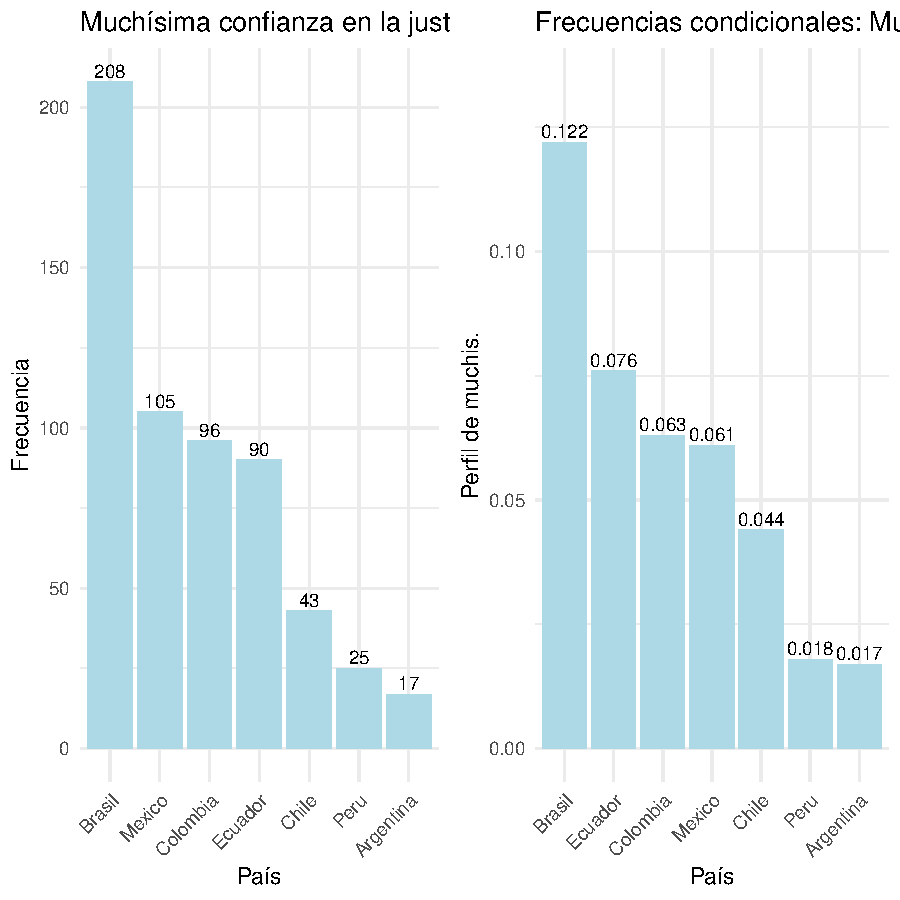
\includegraphics{1_panorama_Diapositivas-019}
\caption{EMV}
\label{fig:EMV_1}
\end{figure}

\end{ejem}

\end{frame}
% 
\begin{frame}[fragile]{Correspondencias simples y análisis de tablas de contingencia \textcolor{magenta}{(EMV)}}
\begin{ejem}
\begin{table}[!h]
\centering
\caption{\label{tab:percol_Cofjust}Perfiles por modalidades de confianza en la justicia respecto a los países encuestados, ordenados por la opción muchísimo}
\centering
\begin{tabular}[t]{lrrrr}
\toprule
  & muchis. & mucho & no\_mucho & nada\\
\midrule
\cellcolor{gray!10}{Brasil} & \cellcolor{gray!10}{0.356} & \cellcolor{gray!10}{0.339} & \cellcolor{gray!10}{0.113} & \cellcolor{gray!10}{0.123}\\
Mexico & 0.180 & 0.140 & 0.155 & 0.234\\
\cellcolor{gray!10}{Colombia} & \cellcolor{gray!10}{0.164} & \cellcolor{gray!10}{0.052} & \cellcolor{gray!10}{0.249} & \cellcolor{gray!10}{0.131}\\
Ecuador & 0.154 & 0.197 & 0.129 & 0.071\\
\cellcolor{gray!10}{Chile} & \cellcolor{gray!10}{0.074} & \cellcolor{gray!10}{0.129} & \cellcolor{gray!10}{0.124} & \cellcolor{gray!10}{0.071}\\
\addlinespace
Peru & 0.043 & 0.055 & 0.109 & 0.259\\
\cellcolor{gray!10}{Argentina} & \cellcolor{gray!10}{0.029} & \cellcolor{gray!10}{0.088} & \cellcolor{gray!10}{0.120} & \cellcolor{gray!10}{0.110}\\
Suma & 1.000 & 1.000 & 1.000 & 1.000\\
\bottomrule
\end{tabular}
\end{table}\end{ejem}
\end{frame}
% 
\begin{frame}[fragile]{Correspondencias simples y análisis de tablas de contingencia \textcolor{magenta}{(EMV)}}
\begin{ejem}
\setkeys{Gin}{width=0.7\textwidth, height=0.5\textheight,keepaspectratio} % para redefinir el tamaño de los graficos
\begin{figure}[H]
	\centering
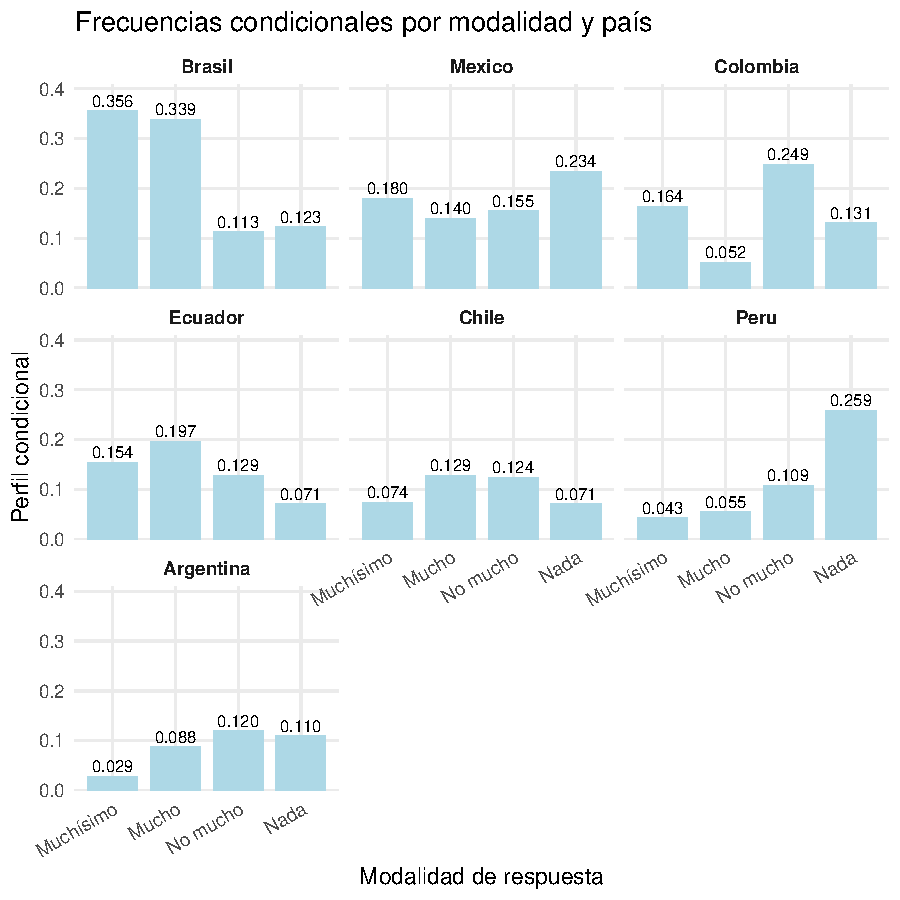
\includegraphics{1_panorama_Diapositivas-021}
\caption{Comparación de países por proporción de respuestas a la percepción de la justicia}
\label{fig:EMV_2}
\end{figure}

\end{ejem}
\end{frame}
% 

\begin{frame}[fragile]{Correspondencias simples y análisis de tablas de contingencia \textcolor{magenta}{(EMV)}}
\begin{ejem}
\setkeys{Gin}{width=0.7\textwidth, height=0.5\textheight,keepaspectratio} % para redefinir el tamaño de los graficos
\begin{figure}[H]
	\centering
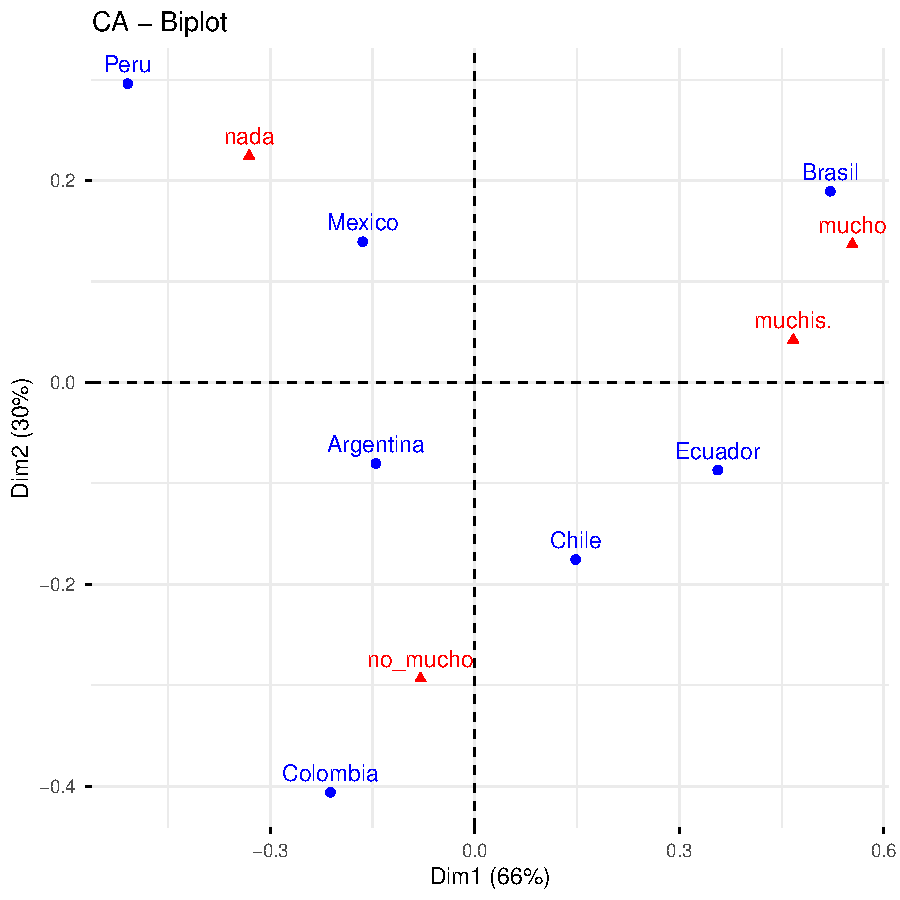
\includegraphics{1_panorama_Diapositivas-023}
\caption{Plano de correspondencias simples que muestra tendencias de los países en cuanto a percepciones sobre confianza en la justicia}
\label{fig:EMV_2}
\end{figure}
\end{ejem}
\end{frame}
% 

\begin{frame}{Correspondencias múltiples: Tablas de tablas de contingencia \textcolor{yellow}{(ECC)}}

\begin{ejem}

\textbf{Encuesta de Cultura Ciudadana}

\vspace{2mm}

La \textbf{Encuesta de Cultura Ciudadana (ECC)} fue realizada por la Corporación
Visionarios en varias ciudades latinoamericanas con cierta periodicidad.
Constituye un instrumento de observación y análisis de distintos aspectos
relacionados con la cultura ciudadana y el comportamiento social.

\end{ejem}

\end{frame}
% 
\begin{frame}{Correspondencias múltiples: Tablas de tablas de contingencia \textcolor{yellow}{(ECC)}}

\begin{ejem}

\textbf{Encuesta de Cultura Ciudadana}

\vspace{2mm}

La encuesta incluye, por ejemplo, preguntas sobre

\begin{itemize}
\item los sentimientos de los encuestados frente a palabras como normas o reglas
(Ley, Moral y Cultura),
\item la facilidad con que pueden actuar conforme a la ley,
\item las capacidades para celebrar y cumplir acuerdos y las reacciones ante su
incumplimiento,
\item pluralismo (aceptación de las diferencias e inclusión),
\item seguridad,
\item confianza interpersonal,
\item confianza en instituciones,
\item victimización, entre otros aspectos.
\end{itemize}

\end{ejem}

\end{frame}
% 

\begin{frame}[fragile]{Correspondencias múltiples: Tablas de tablas de contingencia \textcolor{yellow}{(ECC)}}
\tiny
\begin{ejem}
\newcommand{\ansbox}[1]{\fbox{\rule{0pt}{1.6ex}\hspace{1.2ex}#1\hspace{1.2ex}}}

\begin{table}[H]
\noindent\centering
\setlength{\tabcolsep}{3pt}
\renewcommand{\arraystretch}{1.15}

% (1) Encabezado
\begin{tabularx}{\linewidth}{|>{\raggedright\arraybackslash}X|}
\hline
\textit{20. Dígame si en su opinión se justifica o no desobedecer la ley:} \\
\hline
\end{tabularx}

\vspace{1.5mm}

% (2) Ítems reordenados
\begin{tabularx}{\linewidth}{|
>{\raggedright\arraybackslash}X
>{\centering\arraybackslash}p{1.4cm}
>{\centering\arraybackslash}p{1.4cm}|
>{\raggedright\arraybackslash}X
>{\centering\arraybackslash}p{1.4cm}
>{\centering\arraybackslash}p{1.4cm}|}
\hline
 & \textbf{Sí} & \textbf{No} &  & \textbf{Sí} & \textbf{No} \\
\hline
a.\ Cuando es la única manera de alcanzar sus objetivos
& \ansbox{1} & \ansbox{2}
& g.\ Cuando es bastante seguro que uno no será castigado
& \ansbox{1} & \ansbox{2} \\
\hline
b.\ Cuando es la única manera de ayudarle a la familia
& \ansbox{1} & \ansbox{2}
& h.\ Cuando alguien lo ha hecho y le ha ido bien
& \ansbox{1} & \ansbox{2} \\
\hline
c.\ Cuando es la única manera de luchar públicamente contra una ley o un régimen injusto
& \ansbox{1} & \ansbox{2}
& i.\ Cuando es lo acostumbrado
& \ansbox{1} & \ansbox{2} \\
\hline
d.\ Cuando es muy provechoso económicamente
& \ansbox{1} & \ansbox{2}
& j.\ Para pagar un favor
& \ansbox{1} & \ansbox{2} \\
\hline
e.\ Cuando la creencia religiosa lo permite
& \ansbox{1} & \ansbox{2}
& k.\ Para defender propiedades o bienes
& \ansbox{1} & \ansbox{2} \\
\hline
f.\ Cuando se hace para responder a una ofensa al honor
& \ansbox{1} & \ansbox{2}
&  &  &  \\
\hline
\end{tabularx}
\end{table}
\end{ejem}
\end{frame}
% 


\begin{frame}\textcolor{yellow}{(ECC)}
\begin{ejem}
\setkeys{Gin}{width=0.8\textwidth} % redefinir el tamaño graficos
\begin{figure}[H]
	\centering
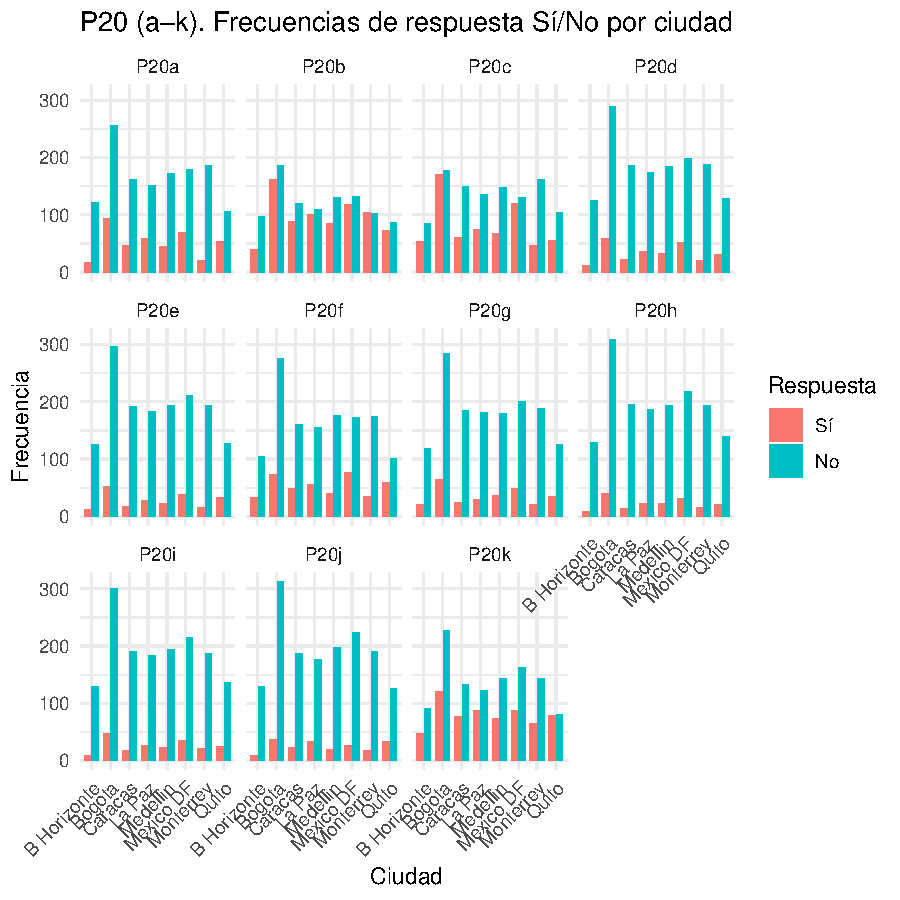
\includegraphics{1_panorama_Diapositivas-026}
	\caption{Frecuencias de respuesta por países. Se observa una tendencia general a no justificar la dsobediencia de la ley: Barras azules mayores que las rojas. Sin embargo, las preguntas P20b, P20c y P20k, muestran mayor cercanía entre Sí y No}\label{fig:justifica_desobe_ley}
\end{figure}
\end{ejem}
\end{frame}
% 
\begin{frame}{\textcolor{yellow}{(ECC)}}
\begin{ejem}
\setkeys{Gin}{width=0.7\textwidth} % redefinir el tamaño graficos
\begin{figure}[H]
	\centering
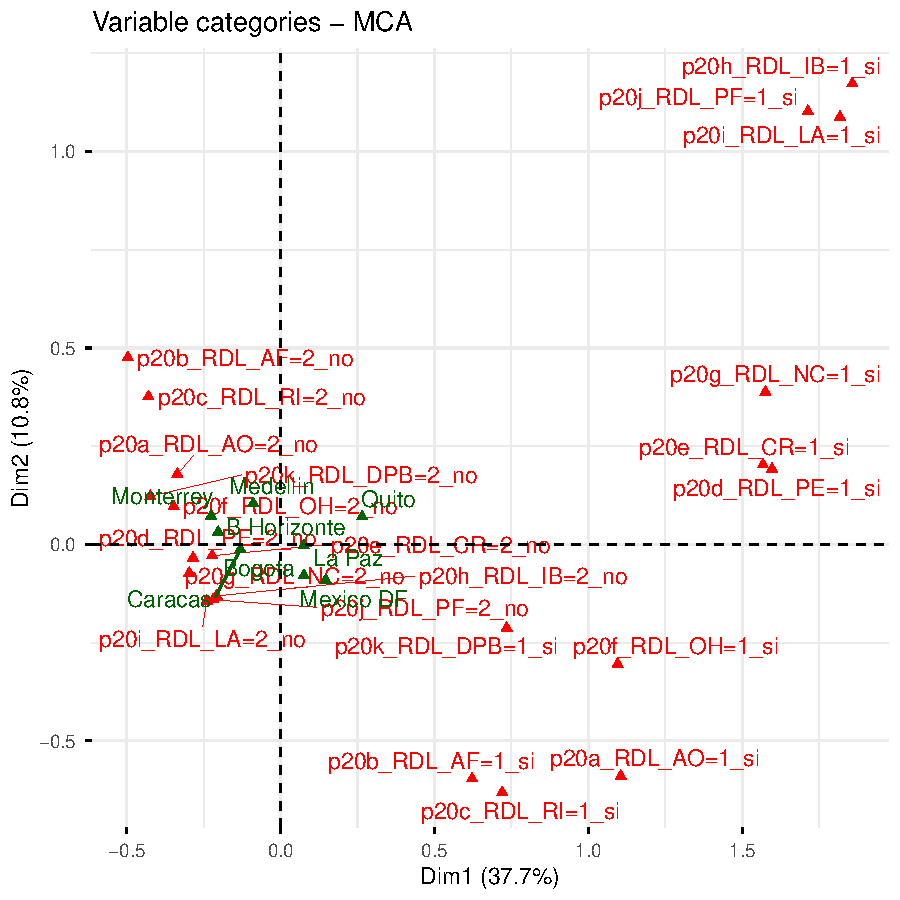
\includegraphics{1_panorama_Diapositivas-027}
	\caption{Tendencias a justificar la desobediencia de la ley por ciudades}\label{fig:Tendencias_just_des_ley}
\end{figure}
\end{ejem}
\end{frame}
% 
% \begin{frame}{\textcolor{yellow}{(ECC)}}
% \begin{ejem}
% \setkeys{Gin}{width=1\textwidth} % redefinir el tamaño graficos
% \begin{figure}[H]
% 	\centering
% <<mca_var_conexiones, echo=F, fig=TRUE, width=7.2, height=4.6>>=
%   library(FactoMineR)
% library(factoextra)
% library(ggplot2)
% library(dplyr)
% 
% # MCA (ciudad como suplementaria: quali.sup = 1)
% res.mca.jdl <- MCA(cclat_p20, quali.sup = 1, graph = FALSE)
% 
% # Base plot
% p <- fviz_mca_var(res.mca.jdl, repel = TRUE)
% 
% # --- Coordenadas de modalidades activas (Dim 1 y Dim 2) ---
% coord <- as.data.frame(res.mca.jdl$var$coord[, 1:2])
% coord$mod <- rownames(coord)
% names(coord)[1:2] <- c("x", "y")
% 
% # --- Ítems a conectar: h, i, j ---
% # Ajuste estos "base" si sus prefijos/códigos difieren
% bases <- c("p20h_RDL_IB", "p20i_RDL_LA", "p20j_RDL_PF")
% 
% # Construir pares Sí/No con los nombres exactos usados por exams/Moodle
% pairs <- data.frame(
%   base = bases,
%   si   = paste0(bases, "=1_si"),
%   no   = paste0(bases, "=2_no"),
%   stringsAsFactors = FALSE
% )
% 
% # Extraer coords para sí/no
% df_si <- coord %>% filter(mod %in% pairs$si) %>% rename(x_si = x, y_si = y)
% df_no <- coord %>% filter(mod %in% pairs$no) %>% rename(x_no = x, y_no = y)
% 
% # Unir por el "base" (haciendo match con los nombres)
% df_lines <- pairs %>%
%   left_join(df_si, by = c("si" = "mod")) %>%
%   left_join(df_no, by = c("no" = "mod"))
% 
% # Verificación rápida: si faltan filas es porque los nombres no coinciden
% if (any(!complete.cases(df_lines[, c("x_si","y_si","x_no","y_no")]))) {
%   warning("No se encontraron todas las modalidades si/no. Revise los nombres en rownames(res.mca.jdl$var$coord).")
% }
% 
% # --- Agregar conexiones punteadas suaves ---
% p +
%   geom_curve(
%     data = df_lines,
%     aes(x = x_si, y = y_si, xend = x_no, yend = y_no),
%     inherit.aes = FALSE,
%     linetype = "dashed",
%     linewidth = 0.6,
%     curvature = 0.25
%   ) +
%   geom_point(
%     data = df_lines,
%     aes(x = x_si, y = y_si),
%     inherit.aes = FALSE,
%     size = 2
%   ) +
%   geom_point(
%     data = df_lines,
%     aes(x = x_no, y = y_no),
%     inherit.aes = FALSE,
%     size = 2
%   )
% @
% 	\caption{Las líneas punteadas representan las formas sinuosas que se mostraron en los histogramas}\label{fig:Tendencias_just_des_ley_1}
% \end{figure}
% \end{ejem}
% \end{frame}
% 
\begin{frame}{Métodos de agrupamiento (Clustering) Sistema universitario estatal (SUE)}
\begin{ejem}
El \textbf{Sistema Universitario Estatal} (SUE) es una red de universidades públicas colombianas, orientada hacia la colaboración académica, la investigación y la gestión conjunta de recursos entre estas ellas. Datos de éstas universidades se recolectan en una tabla que contiene 32 indicadores de educación superior para 32 universidades estatales entre 2003 y 2012.
\end{ejem}
\end{frame}
% 
\begin{frame}{Métodos de agrupamiento (Clustering) Sistema universitario estatal (SUE)}
\begin{ejem}
Para este ejemplo se utilizan seis indicadores:

\begin{itemize}
\item Docentes de tiempo completo o equivalente (DCTC2012),
\item gastos en personal administrativo (GPA2012),
\item matrícula de pregrado (MPRE2012),
\item matrícula de posgrado (MPOS2012),
\item graduados de pregrado (GrPre2012),
\item graduados de posgrado (GrPos2012).
\end{itemize}

En la Tabla~\ref{tab:sue} se presentan los valores de estos indicadores para las 32 universidades públicas.
\end{ejem}
\end{frame}
% 


% 
\begin{frame}{Métodos de agrupamiento (Clustering) Sistema universitario estatal (SUE)}
\begin{ejem}
\begin{table}[!h]
\centering
\caption{\label{tab:sue}Indicadores del SUE para 32 universidades públicas en el año 2012}
\centering
\resizebox{\ifdim\width>\linewidth\linewidth\else\width\fi}{!}{
\begin{tabular}[t]{lrrrrrr}
\toprule
  & DCTC2012 & GPA2012 & MPRE2012 & MPOS2012 & GrPre2012 & GrPos2012\\
\midrule
\cellcolor{gray!10}{NACIONAL} & \cellcolor{gray!10}{2161} & \cellcolor{gray!10}{347233353} & \cellcolor{gray!10}{42120} & \cellcolor{gray!10}{9299} & \cellcolor{gray!10}{4903} & \cellcolor{gray!10}{3181}\\
PEDAGOGICA & 440 & 7986738 & 9321 & 1614 & 1186 & 362\\
\cellcolor{gray!10}{UPTC} & \cellcolor{gray!10}{828} & \cellcolor{gray!10}{20641880} & \cellcolor{gray!10}{24644} & \cellcolor{gray!10}{2360} & \cellcolor{gray!10}{3190} & \cellcolor{gray!10}{1225}\\
CAUCA & 550 & 28539431 & 12859 & 700 & 1372 & 303\\
\cellcolor{gray!10}{TEC DE PEREIRA} & \cellcolor{gray!10}{442} & \cellcolor{gray!10}{15343348} & \cellcolor{gray!10}{15423} & \cellcolor{gray!10}{1319} & \cellcolor{gray!10}{1532} & \cellcolor{gray!10}{299}\\
\addlinespace
CALDAS & 418 & 12877924 & 12261 & 971 & 1953 & 266\\
\cellcolor{gray!10}{CORDOBA} & \cellcolor{gray!10}{336} & \cellcolor{gray!10}{17354987} & \cellcolor{gray!10}{12081} & \cellcolor{gray!10}{377} & \cellcolor{gray!10}{809} & \cellcolor{gray!10}{0}\\
SURCOLOMBIANA & 284 & 10982676 & 9867 & 435 & 1113 & 265\\
\cellcolor{gray!10}{AMAZONIA} & \cellcolor{gray!10}{198} & \cellcolor{gray!10}{6113236} & \cellcolor{gray!10}{6851} & \cellcolor{gray!10}{332} & \cellcolor{gray!10}{724} & \cellcolor{gray!10}{177}\\
MILITAR & 375 & 10673047 & 12850 & 2678 & 978 & 1218\\
\addlinespace
\cellcolor{gray!10}{TEC DEL CHOCO} & \cellcolor{gray!10}{240} & \cellcolor{gray!10}{21314583} & \cellcolor{gray!10}{10668} & \cellcolor{gray!10}{43} & \cellcolor{gray!10}{1536} & \cellcolor{gray!10}{49}\\
LLANOS & 201 & 13159385 & 5218 & 267 & 653 & 136\\
\cellcolor{gray!10}{POPU DEL CESAR} & \cellcolor{gray!10}{184} & \cellcolor{gray!10}{5206608} & \cellcolor{gray!10}{13127} & \cellcolor{gray!10}{0} & \cellcolor{gray!10}{1653} & \cellcolor{gray!10}{159}\\
MAY DE CNAMARCA & 203 & 7597155 & 5028 & 235 & 870 & 237\\
\cellcolor{gray!10}{PACIFICO} & \cellcolor{gray!10}{65} & \cellcolor{gray!10}{3613371} & \cellcolor{gray!10}{2115} & \cellcolor{gray!10}{0} & \cellcolor{gray!10}{128} & \cellcolor{gray!10}{0}\\
\addlinespace
ANTIOQUIA & 1848 & 71634254 & 36788 & 2760 & 3437 & 815\\
\cellcolor{gray!10}{ATLANTICO} & \cellcolor{gray!10}{371} & \cellcolor{gray!10}{11693780} & \cellcolor{gray!10}{19907} & \cellcolor{gray!10}{255} & \cellcolor{gray!10}{1559} & \cellcolor{gray!10}{151}\\
VALLE & 935 & 61192000 & 26245 & 3238 & 3209 & 800\\
\cellcolor{gray!10}{UIS} & \cellcolor{gray!10}{632} & \cellcolor{gray!10}{49145313} & \cellcolor{gray!10}{19897} & \cellcolor{gray!10}{1869} & \cellcolor{gray!10}{2726} & \cellcolor{gray!10}{607}\\
CARTAGENA & 435 & 44876932 & 18804 & 861 & 1236 & 320\\
\addlinespace
\cellcolor{gray!10}{NARINO} & \cellcolor{gray!10}{296} & \cellcolor{gray!10}{9449989} & \cellcolor{gray!10}{11099} & \cellcolor{gray!10}{549} & \cellcolor{gray!10}{1208} & \cellcolor{gray!10}{270}\\
TOLIMA & 321 & 23307867 & 37080 & 1183 & 4499 & 577\\
\cellcolor{gray!10}{QUINDIO} & \cellcolor{gray!10}{437} & \cellcolor{gray!10}{13088429} & \cellcolor{gray!10}{15740} & \cellcolor{gray!10}{140} & \cellcolor{gray!10}{2051} & \cellcolor{gray!10}{45}\\
UFPS\_CUCUTA & 288 & 7109593 & 20528 & 555 & 2273 & 200\\
\cellcolor{gray!10}{UFPS\_OCANA} & \cellcolor{gray!10}{56} & \cellcolor{gray!10}{3881551} & \cellcolor{gray!10}{4588} & \cellcolor{gray!10}{57} & \cellcolor{gray!10}{307} & \cellcolor{gray!10}{43}\\
\addlinespace
PAMPLONA & 525 & 9552468 & 23887 & 317 & 5320 & 315\\
\cellcolor{gray!10}{MAGDALENA} & \cellcolor{gray!10}{307} & \cellcolor{gray!10}{4944457} & \cellcolor{gray!10}{20082} & \cellcolor{gray!10}{613} & \cellcolor{gray!10}{2910} & \cellcolor{gray!10}{345}\\
CUNDINAMARCA & 309 & 11632868 & 10432 & 107 & 1064 & 171\\
\cellcolor{gray!10}{SUCRE} & \cellcolor{gray!10}{116} & \cellcolor{gray!10}{3997130} & \cellcolor{gray!10}{4838} & \cellcolor{gray!10}{66} & \cellcolor{gray!10}{678} & \cellcolor{gray!10}{0}\\
GUAJIRA & 224 & 9381315 & 7962 & 277 & 696 & 0\\
\addlinespace
\cellcolor{gray!10}{DISTRITAL} & \cellcolor{gray!10}{758} & \cellcolor{gray!10}{16043464} & \cellcolor{gray!10}{27293} & \cellcolor{gray!10}{1696} & \cellcolor{gray!10}{2974} & \cellcolor{gray!10}{683}\\
UNAD & 743 & 14683191 & 64558 & 1678 & 2106 & 124\\
\bottomrule
\end{tabular}}
\end{table}
\end{ejem}
\end{frame}
% 

% ======================================
%========================================
\begin{frame}{DCTC (1/2)}


\setkeys{Gin}{width=\textwidth}
\begin{figure}[H]
\centering
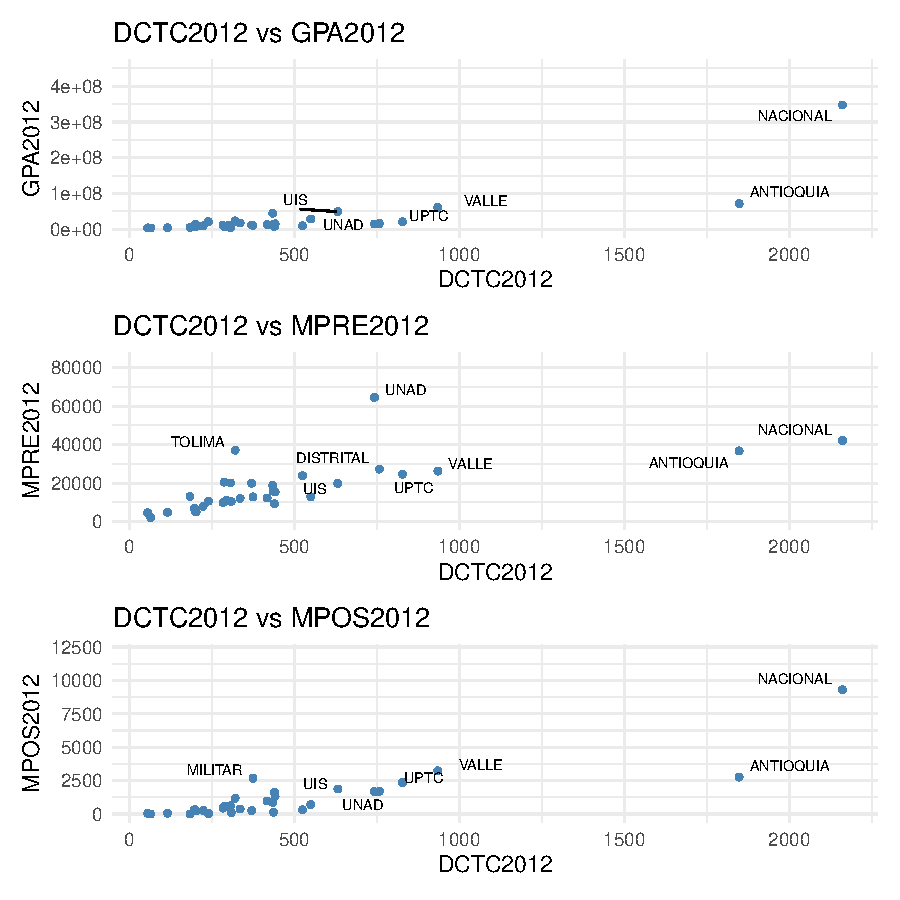
\includegraphics{1_panorama_Diapositivas-032}
\caption{Docentes de tiempo completo o equiv. vs. los otros indicadores del SUE}
\label{dtce_1}
\end{figure}
\end{frame}

%========================================
\begin{frame}{DCTC (2/2)}
\centering
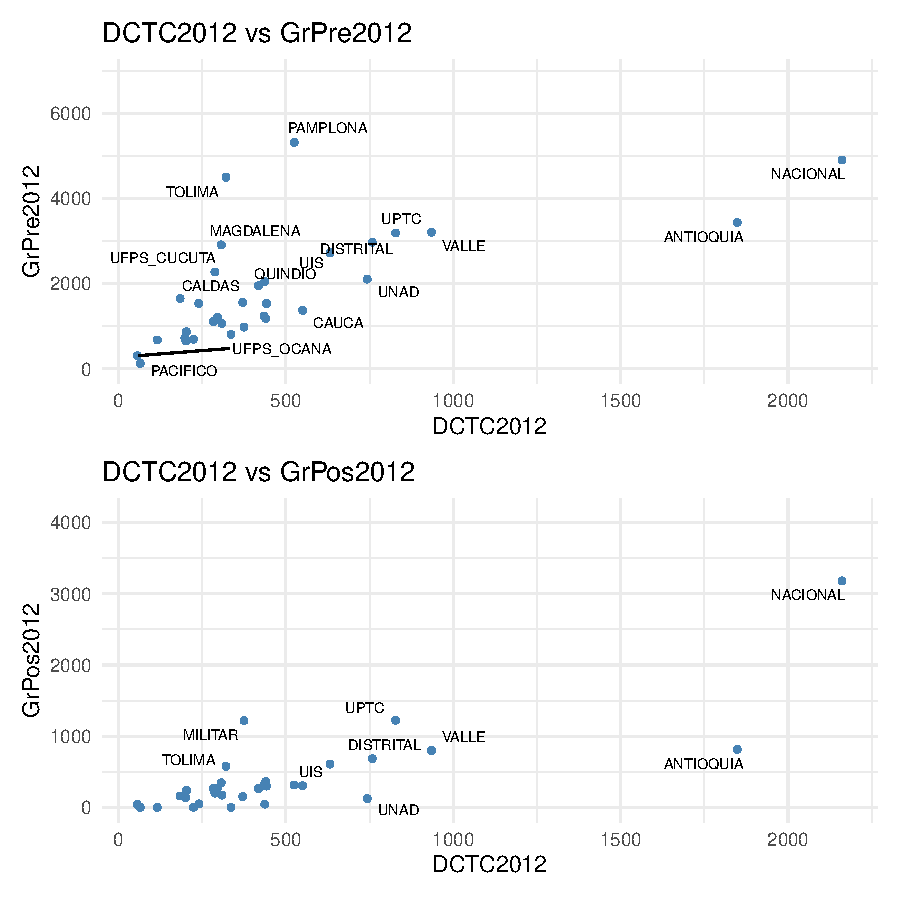
\includegraphics{1_panorama_Diapositivas-033}
\end{frame}

%========================================
\begin{frame}{GPA (1/2)}
\centering
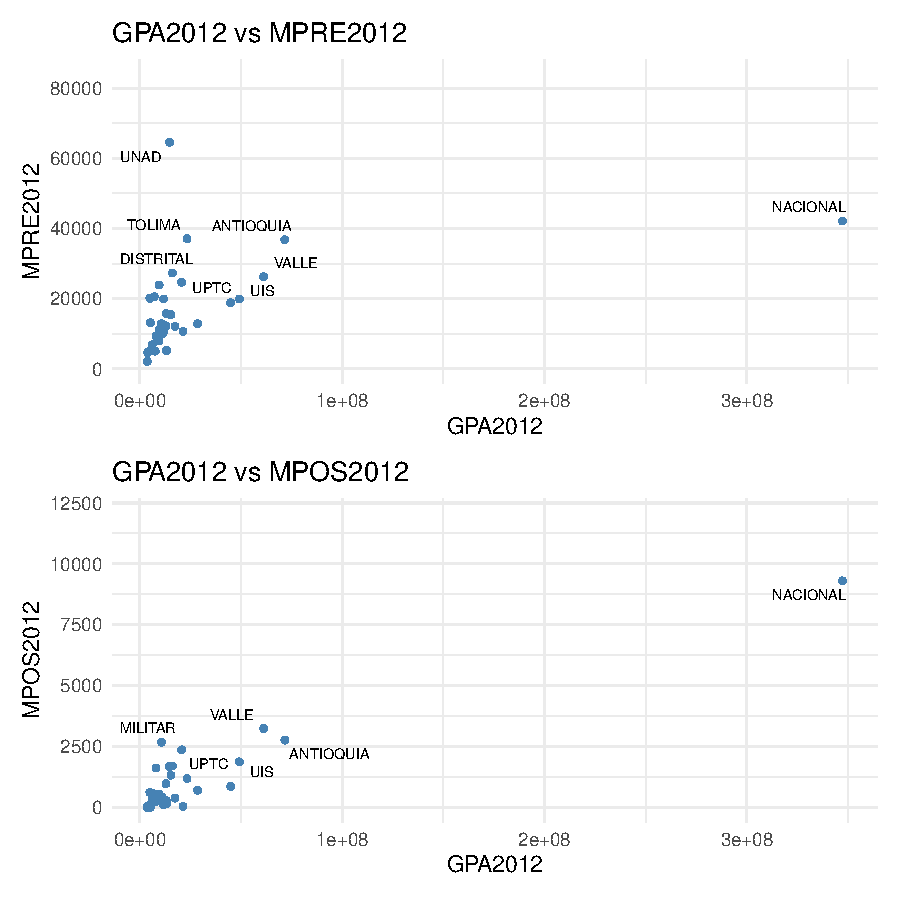
\includegraphics{1_panorama_Diapositivas-034}
\end{frame}

%========================================
\begin{frame}{GPA (2/2)}
\centering
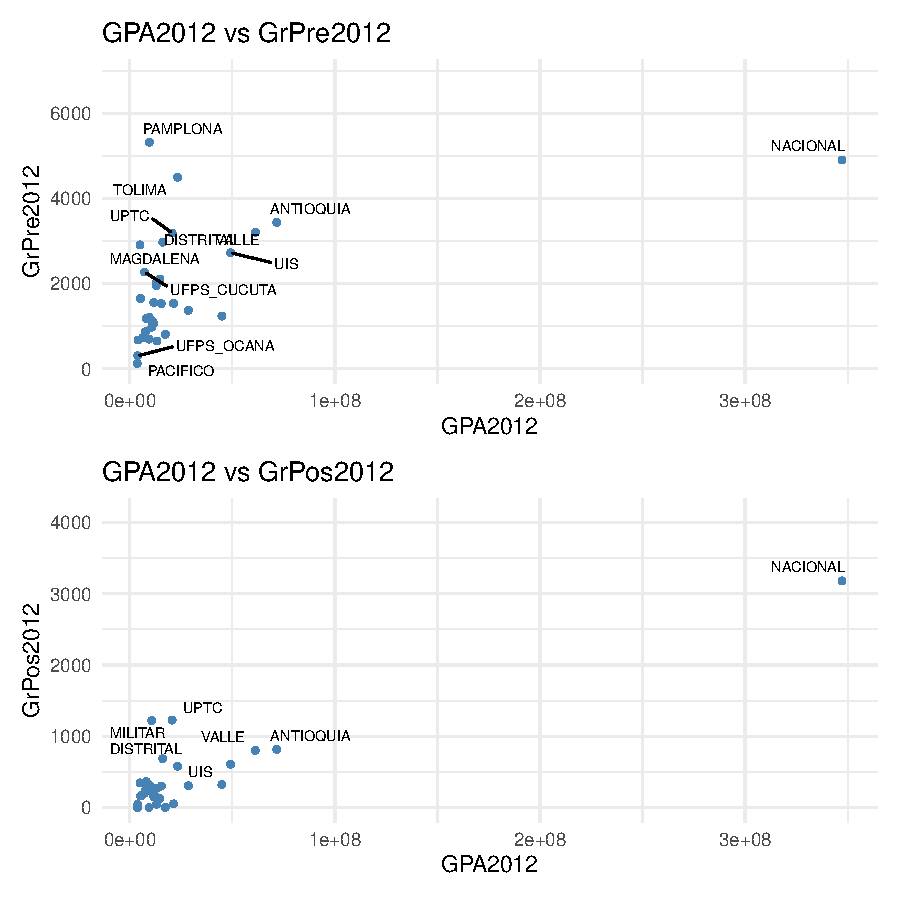
\includegraphics{1_panorama_Diapositivas-035}
\end{frame}

%========================================
\begin{frame}{Indicadores (10--12)}
\centering
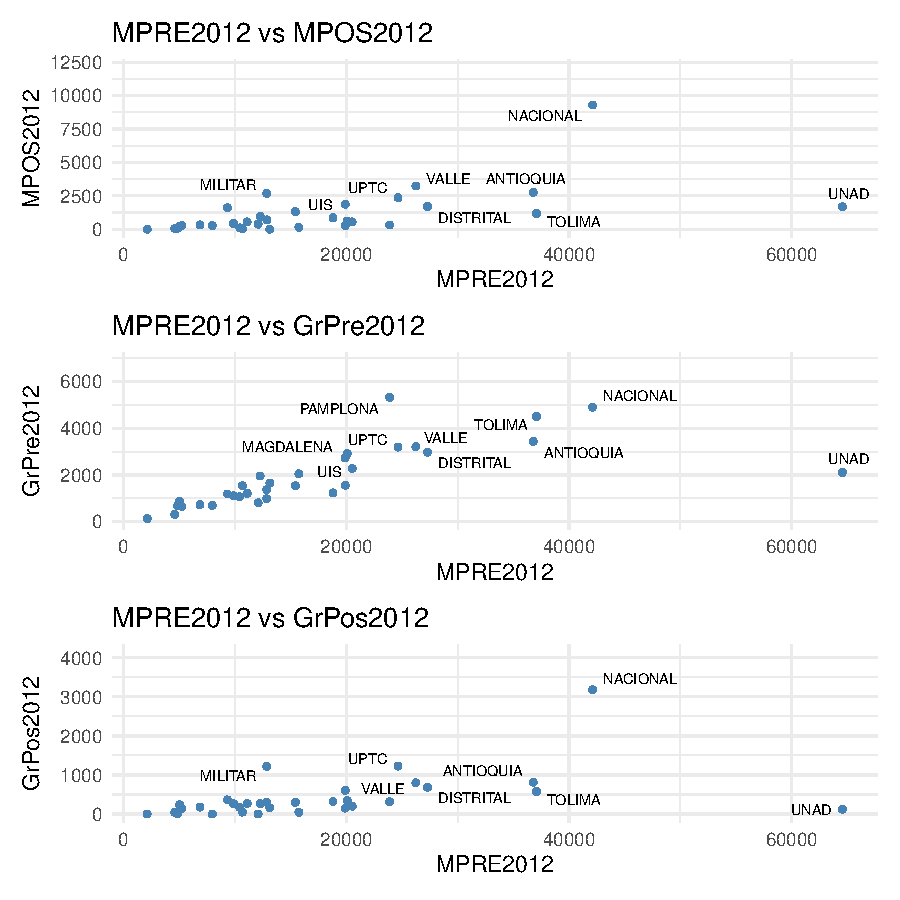
\includegraphics{1_panorama_Diapositivas-036}
\end{frame}

%========================================
\begin{frame}{Indicadores (13--14)}
\centering
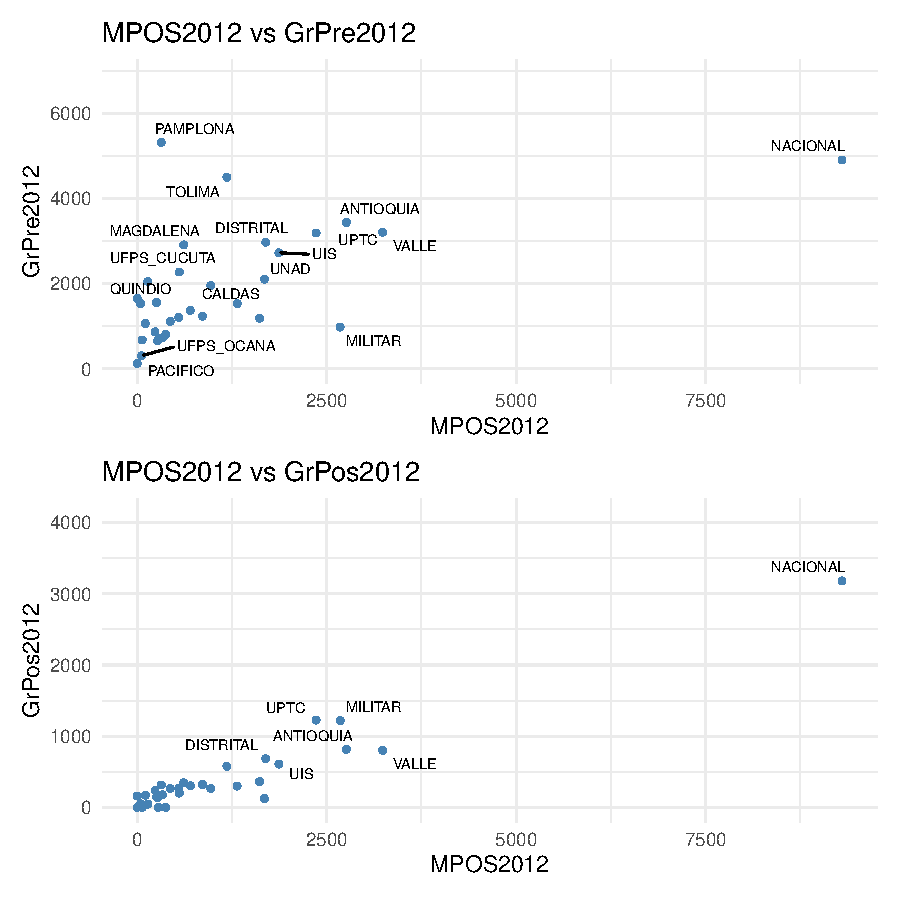
\includegraphics{1_panorama_Diapositivas-037}
\end{frame}

%========================================
\begin{frame}{Indicador (15)}
\centering
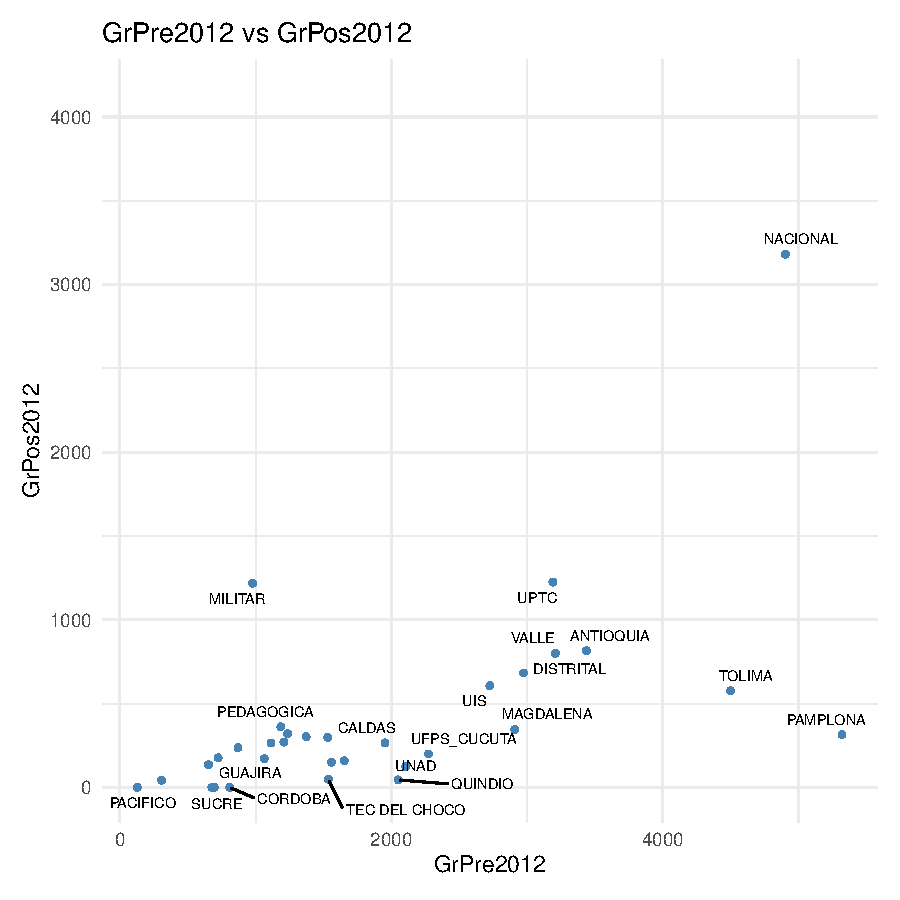
\includegraphics{1_panorama_Diapositivas-038}
\end{frame}

% 
\begin{frame}
\begin{ejem}
\setkeys{Gin}{width=0.6\textwidth, height=0.5\textheight,keepaspectratio} % para redefinir el tama?o de los graficos
\begin{figure}[H]
\centering
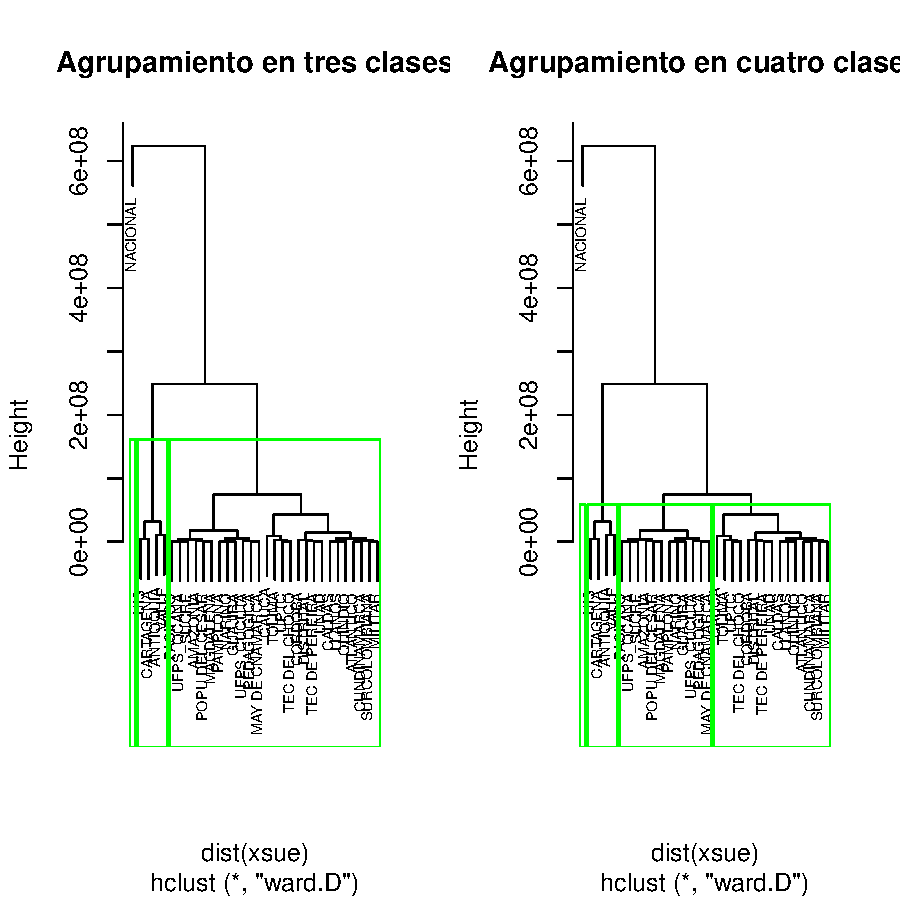
\includegraphics{1_panorama_Diapositivas-040}
\caption{Agrupamiento de universidades del SUE en cuatro grupos}\label{fig:dendroUnis4G}
\end{figure}
\end{ejem}
\end{frame}
% 
% Plano 1-2
\begin{frame}
\begin{ejem}
\setkeys{Gin}{width=0.6\textwidth, height=0.5\textheight,keepaspectratio} % para redefinir el tama?o de los graficos
\begin{figure}[H]
\centering
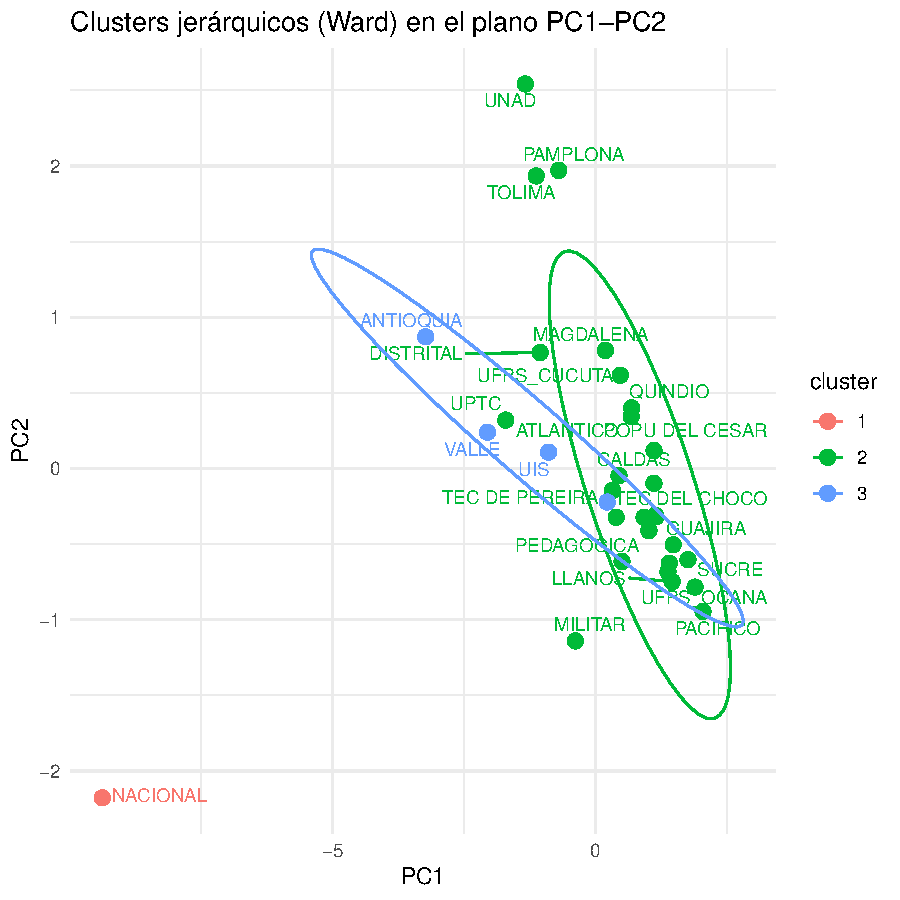
\includegraphics{1_panorama_Diapositivas-041}
\caption{Agrupamiento de universidades del SUE en tres grupos}\label{fig:plano_1_2}
\end{figure}
\end{ejem}
\end{frame}

\end{document}
